\chapter{Evaluation and Analysis}
\label{chap:evaluation}

In this chapter, we present our evaluation, findings, and analysis of our method, the KryBall optimisation algorithm. We start by discussing the implementation of KryBall in \ref{sec:implementation}. We then present the experimental setup in \ref{sec:experimental_setup}, which includes the datasets, models, metrics, hyperparameter settings, and tasks to be evaluated. This is followed by our results in \ref{sec:results}, where we include our empirical evaluations and sensitivity analysis. We then interpret our findings and do some further analysis in \ref{sec:discussion_and_further_analysis}. Finally, we discuss the limitations of our method in \ref{sec:limitations}.

\section{Implementation}
\label{sec:implementation}

Most machine learning workflows and tasks are implemented entirely in Python, and leverage the PyTorch library. This is because PyTorch has efficient low-level kernels and bindings that allow for automatic differentation and tensor operations. We design our optimiser to be integrated seamlessly with PyTorch. As such, KryBall can act as a drop-in replacement for other PyTorch optimisers in deep learning tasks.

\subsection{Adhering to the PyTorch Optimiser API}
\label{ssec:adhering_to_the_pytorch_optimiser_api}

Our implementation adheres to the PyTorch optimiser API while simplifying the standard training workflow. In a typical training setup in PyTorch, users must explicitly call the following functions:
\begin{itemize}
    \item \verb|.backward()| to create the computation graph and the associated gradients.
    \item \verb|.zero_grad()| to clear previous gradients.
    \item \verb|.step()| to perform the optimisation step and update the model parameters.
\end{itemize}
We instead consolidate these into just a single \verb|step| function. This makes it cleaner than the current workflow while maintaining full compatibility with the PyTorch ecosystem. This results in a more clean implementation for end users that reduces boilerplate code. 

In addition, we provide an interpretable way to track necessary information. In PyTorch, optimiser parameters such as momentum and adaptive learning rates are associated with individual parameter blocks and buried within the optimiser's internal state dictionaries. This makes it difficult to understand how they behave during training. Our implementation exposes these quantities directly as accessible vectors, allowing researchers to easily inspect gradients, momentum terms, and other optimisation variables. This facilitates deeper insights into the optimisation process and enables more effective understanding and debugging.

\subsection{Function Integration with PyTorch}
\label{ssec:function_integration_with_pytorch}

We also introduce a novel test suite that integrates classic functions (Rosenbrock, 2D Saddle, Monkey Saddle etc.) with PyTorch. Currently, most existing implementations that offer direct optimisation of just functions do not integrate with PyTorch. Instead, they all use numerical solvers and approximate the first and second-order derivatives. This is because PyTorch workflows are primarily for deep learning, and simple function optimisation is not a focus. To our knowledge, there exists only a few libraries that try and integrate function optimisation with deep learning. However, these are outdated, lack maintainability, and do not use modern PyTorch techniques such as model JIT compilation to improve speed. We thus implement an easy way to optimise any function with PyTorch optimisers such as SGD, Adam and LBFGS that adheres to the standard training loop. We show an example in \cref{alg:optimise_function_with_pytorch}.

\begin{algorithm}[h]
    \small
    \DontPrintSemicolon
    T = 100\;
    model = Rosenbrock()\;
    optimiser = torch.optim.LBFGS(model.parameters())\;
    \For{$t=1, 2, \ldots, T$}{
        optimiser.zero\_grad()\;
        loss = model()\;
        loss.backward()\;
        optimiser.step()\;
    }
    \caption{Optimising a function with PyTorch optimisers}
    \label{alg:optimise_function_with_pytorch}
\end{algorithm}


\subsection{The Trust-Region Framework}
\label{ssec:the_trust_region_framework}

A core contribution that we present is a novel implementation of $N$-dimensional subspace optimisation that solves the trust-region subproblem. To our knowledge, this is the first general-purpose implementation tailored for deep learning applications within the PyTorch ecosystem. Many trust-region frameworks either employ the dogleg method, or 2D subspace optimisation, but also are not integrated with PyTorch. We thus implement a general-purpose $N$-dimensional subspace optimiser that can be used with any PyTorch optimiser, and more generally any task that involves the trust-region subproblem. 

\subsection{Loss Landscape Sampling}
\label{ssec:loss_landscape_sampling}

The final part of our contributions that we implement is the ability to inspect the loss landscape of deep learning training tasks. We implement a sampler that can be used to sample trajectories from the loss landscape of a deep learning model. Given a particular point in training, our sampler can investigate the local geometry by performing an exhaustive line search along the optimiser's step direction. This allows researchers to visualise and analyse the characteristics of the loss landscape in the vicinity of the optimisation trajectory for a particular optimiser. To our knowledge, this has not been done before, and we use this to analyse the trajectory of optimisers for different deep learning tasks in \cref{sec:discussion_and_further_analysis}. This inspection tool enables deeper insights into optimisation dynamics, and can help explain why certain optimisers perform better on specific tasks, and at which points in training they suffer.

\section{Experimental Setup}
\label{sec:experimental_setup}
% Introduction to this section
To evaluate KryBall, we must first define a diverse range of tasks that accurately reflect the challenges faced by deep learning models. In this section, we define these tasks with respect to the datasets, models, metrics, and hyperparameter tuning setups. We consider the following tasks as our suite: ill-conditioned functions, binary classification, and image classification. Our optimiser suite primarily consists of the MSGD and Adam, which were introduced in \cref{chap:lit_review}, and our KryBall optimiser. 

\subsection{Baselines}
\label{ssec:baselines}
Before we introduce our tasks, we first define our baselines. We select MSGD and Adam as our baseline optimisers. These are state-of-the-art first-order optimisers that we find outcompetes other optimisers in literature. MSGD is a simple and foundational approach that is well-suited for many deep learning tasks. Adam is more of a modern and practical baseline, and has been the standard optimiser in practice ever since it was introduced. We also use LBFGS as a second-order baseline, as it exhibits good performance across many tasks and is also a popular optimiser in practice. However, we note that we only use LBFGS where it is tractable, and so for the image classification task in \cref{ssec:task_3_image_classification}, we do not use LBFGS to remain consistent.

\subsection{Task 1: Ill-Conditioned Function Optimisation}
\label{ssec:task_1_ill_conditioned_function_optimisation}
The first set of tasks involves minimising ill-conditioned objective functions. We choose the Rosenbrock function and implement a noisy, stochastic variant of it, and the Rahimi-Recht function, which we briefly mentioned in \cref{sssec:ill_conditioning} of \cref{chap:background}.

% TODO: Cite properly
\subsubsection{Stochastic Rosenbrock Function}
\label{sssec:task_1_rosenbrock_function}
We implement a stochastic variant of the Rosenbrock function from \cite{NoceWrig06}. We have that $\mathcal{R}: \mathbb{R}^2 \rightarrow \mathbb{R}$:
\begin{equation}
\mathcal{R}(x, y) = (1 - x)^2 + 100\epsilon_i(y - x^2)^2,
\end{equation}
where at each evaluation of the function, a noise sample $\epsilon_i$ is drawn from a uniform distribution $\mathcal{U}[\lambda_1, \lambda_2]$ with $\lambda_1 \leq \lambda_2$. When $\lambda_1 = \lambda_2 = 1$, we can recover the deterministic Rosenbrock function with its well-known minimum at $(x, y) = (1, 1)$. To assess robustness to noise, we compare each optimiser on both the deterministic formulation and two stochastic variants with different noise regimes.

% TODO: Cite Henriques and Rahimi and Recht
\subsubsection{Rahimi-Recht Function}
\label{sssec:task_1_rahimi_recht_function}
The second function is an ill-conditioned linear regression problem introduced by Rahimi and Recht. This involves training a neural network with two linear layers to approximate a linear map with a high condition number. The objective function is
\begin{equation}
\mathcal{L}(W) = \|\hat{y} - y_{true}\|^2 = \|W_L W_{L-1} \cdots W_1 x - Ax\|^2, 
\end{equation}
where $A$ is an ill-conditioned matrix with condition number $\kappa$, and $W_i$ are the weight matrices of the linear network. We construct the true linear map $A_{true} \in \mathbb{R}^{m \times d}$ with singular values linearly spaced between 1 and $\kappa$. We generate $n=1000$ random input samples and compute the corresponding outputs using this map. The behaviour of this function is that as we get closer to the minima, it becomes increasingly ill-conditioned. Specifically, the eigenvalues of the Hessian tend towards infinity.

\subsubsection{Evaluation Setup and Metrics}
\label{sssec:task_1_evaluation_setup_and_metrics}
We evaluate MSGD, Adam, LBFGS, and KryBall on the Rosenbrock and the Rahimi-Recht functions with the following chosen ill-conditioning parameters:
\begin{itemize}
    \item \textbf{Deterministic Rosenbrock}: $\lambda_1 = \lambda_2 = 1$.
    \item \textbf{Stochastic Noisy Rosenbrock}: $\lambda_1 = 0$, $\lambda_2 = 1$.
    \item \textbf{Stochastic Noisy Rosenbrock}: $\lambda_1 = 0$, $\lambda_2 = 3$.
    \item \textbf{Slightly Ill-Conditioned Rahimi-Recht}: $\kappa = 10$.
    \item \textbf{Highly Ill-Conditioned Rahimi-Recht}: $\kappa = 1e5$.
\end{itemize}
Each optimiser is tuned using Hyperband on each function for 20 sweeps, where each sweep has 100 epochs. We describe in detail our hyperparameter tuning setup in \cref{ssec:hyperparameter_tuning_setup}. We then use the best performing configuration for each optimiser, and then run all optimisers with a budget of 2000 epochs until they converge within an $\epsilon$ of the solution or use up the computational budget. For Rosenbrock, we choose $\epsilon = 1 \times 10^{-4}$ and for Rahimi-Recht we choose $\epsilon = 1 \times 10^{-2}$. Here, we are measuring the optimisers ability to converge to the solution while handling noise and ill-conditioning.

\subsection{Task 2: XOR Classification}
\label{ssec:task_2_xor_classification}

The next task we consider is a simple case of binary classification with the XOR function. This is a good task to bridge between the ill-conditioned functions and more complex recognition tasks as it introduces non-linearity. The XOR task cannot be linearly separated, and needs a non-linear activation function. Our dataset is simple and small. It includes all 4 combinations of inputs to the XOR function, a 2D vector of zeros and ones, and the corresponding labels in which they evaluate to.

\subsubsection{Evaluation Setup and Metrics}
\label{sssec:task_2_evaluation_setup_and_metrics}
% TODO: Reference BCE
For this task, we use a simple MLP with 3 layers, consisting of one input layer, a hidden layer with a hidden dimension of size 8, and an output layer. Our activation function is the Softplus function, and our loss function is the Binary Cross Entropy (BCE) loss. The BCE loss is defined as
\begin{equation}
\mathcal{L}(y, \hat{y}) = -\frac{1}{N} \sum_{i=1}^N \left[ y_i \log \hat{y}_i + (1 - y_i) \log (1 - \hat{y}_i) \right],
\end{equation}
and measures the difference between the predicted probability distribution and the actual distribution which consists of the ground truth labels for a binary classification task. This is useful for the XOR case since our output is binary.

We test MSGD, Adam, LBFGS, and KryBall on this task. Each optimiser is tuned for 20 sweeps, each with 100 epochs like the previous task. We use the best performing parameters, and then run each optimiser on the XOR task with a budget of 100 epochs. Given this task is quite simple, and our chosen model is more than capable, we measure the number of epochs it takes to converge. Our convergence criteria here is to reach perfect accuracy, that is an accuracy of 1.0, and completely minimise the loss function (reach 0 loss). This means we have perfectly predicted the XOR problem. In practice, most models and most optimisers are capable of this, and thus we instead focus on convergence speed. 

\subsection{Task 3: Image Classification}
\label{ssec:task_3_image_classification}

Our third and final task is a suite of image classification problems. Here, given an image $I$ that is usually either a binary image or an RGB image, we want to classify it into one of $C$ classes. We thus use a variety of datasets to formulate our image classification problem.

\subsubsection{MNIST-1D}
\label{sssec:task_3_mnist_1d}
MNIST-1D is a scaled down one-dimensional version analogue of the classic MNIST handwritten digit dataset \citep{greydanus_mnist1d}. It consists of 40-dimensional time series signals that represent the handwritten digits from 0 to 9. These are constructed through procedural generation and involve random transformations such as padding, translation and scaling operations \citep{greydanus_mnist1d}. There are 5000 total samples in MNIST-1D, where 4000 are allocated for training and 1000 for testing \citep{greydanus_mnist1d}. Each example in MNIST-1D is labeled with its corresponding digit class (0--9). This estbalishes a 10-class classification problem where the ground truth represents the original digit template from which each signal was derived.

\subsubsection{CIFAR-10}
\label{sssec:task_3_cifar_10}
CIFAR-10 is widely used dataset for image classification. It consists of 60000 RBG images that are of size $32 \times 32 \times 3$ \citep{cifar10}. These are distributed across 10 distinct object classes: irplane, automobile, bird, cat, deer, dog, frog, horse, ship, and truck. The dataset comprises 50000 training images and 10000 test images \citep{cifar10}. Each class contains exactly 6000 images, where the train and test split is 5000 and 1000 respectively. The ground truth for this dataset is a single-label classification that indicates the primary object category present in each image \citep{cifar10}. In CIFAR-10, all images are labelled. We note that a superset of CIFAR-10 is CIFAR-100, which instead contains 100 classes. 

\subsubsection{Evaluation Setup and Metrics}
We evaluate our optimisers on the MNIST-1D and CIFAR-10 datasets. We categorise our experiments into three different groups which are based on the model we use. We now describe each of these groups.

\begin{itemize}
    \item \textbf{MNIST-1D MLP}: We use the simple MLP we had from the XOR task. Here, we modify the hidden dimension to be of size 256. This is consistent with the original implementation for MNIST-1D in \citep{greydanus_mnist1d}, and offers a good baseline for this task.
    \item \textbf{CIFAR-10 CNN}: The first model we use to evaluate on CIFAR-10 is a 3-layer Convolutional Neural Network (CNN) with 2 fully connected layers. Here, we use three convolutional layers with 32, 32 and 64 output channels, each using $5 \times 5$ kernels with padding. Each convolution is followed by batch normalisation, our choice of activation and average pooling. We then follow with two fully connected layers to predict out output.
    \item \textbf{CIFAR-10 ResNet-18}: We also evaluate using a stronger model, a ResNet-18, introduced by \citep{resnet}. This deeper architecture employs residual connections to enable training of networks with 18 layers, where each layer consists of four residual blocks with skip connections. ResNet-18 is a baseline architecture for CIFAR-10, and offers good performance in which we can evaluate our optimisers on. 
\end{itemize}
For each model, we use the Softplus activation as done previously. 

For this image classification task, we employ the Categorical Cross Entropy (CCE) loss function. This generalises the BCE loss to multi-class classification problems, extending it to handle $C$ classes. This is done by comparing the predicted probability distribution over all classes with the true one-hot encoded label distribution. The CCE loss is defined as
\begin{equation}
\mathcal{L}(y, \hat{y}) = -\frac{1}{N} \sum_{i=1}^N \sum_{c=1}^C y_{i,c} \log \hat{y}_{i,c}.
\end{equation}
Here, $N$ is the number of samples, $C$ is the number of classes, and $y_{i,c}$ is the true label, where it is 1 if sample $i$ belongs to class $c$ or 0 otherwise, and $\hat{y}_{i,c}$ is the predicted probability for sample $i$ belonging to class $c$. CCE measures the difference between the predicted probability distribution and the actual distribution. This makes it well-suited for CIFAR-10 with given its 10 distinct object categories.

Our metrics for this task are the test accuracy and the training loss. Specifically, we look at the peak test accuracy and final test accuracy achieved during training. We also consider the final training. This shows how well our optimiser is able to train these different models on different datasets.

\subsubsection{Training Setup}
\label{sssec:task_3_training_setup}

Our training setup is distinct from other tasks. Here, we sample mini-batches during training since evaluating on the whole dataset is infeasible. This is unlike our previous tasks, which were not highly parameterised. We now detail the batch size and the number of epochs for each task.
\begin{itemize}
    \item \textbf{MNIST-1D MLP}: The batch size is 512 and we train for 100 epochs.
    \item \textbf{CIFAR-10 CNN}: The batch size is 256 and we train for 40 epochs.
    \item \textbf{CIFAR-10 ResNet-18}: The batch size is 128 and we train for 40 epochs.
\end{itemize}

\subsection{Hyperparameter Tuning Setup}
\label{ssec:hyperparameter_tuning_setup}

All of our experiments are tuned with Bayesian hyperparameter search combined with the Hyperband early stopping algorithm. Hyperband is a bandit-based algorithm that allocates resources to promising configurations while eliminating poorly performing ones early in training. We choose a halving factor $\eta = 3$, which eliminates the worst-performing configurations, retaining only the top $\frac{1}{3}$ of candidates at each successive halving round. This significantly reduces computational cost by avoiding full training of suboptimal hyperparameter combinations. We set a minimum iteration threshold of 10 epochs before any configuration can be terminated, ensuring sufficient training time for meaningful performance evaluation.

\begin{itemize}
    \item \textbf{MSGD}: Learning rate $\alpha \in [1 \times 10^{-4}, 1]$ under a log uniform distribution, momentum $\beta \in [0.8, 0.99]$ under a uniform distribution.
    \item \textbf{Adam}: Learning rate $\alpha \in [1 \times 10^{-4}, 1]$ under a log uniform distribution, betas $\beta_1 \in [0.9, 0.999]$ and $\beta_2 \in [0.99, 0.99999]$ under a uniform distribution.
    \item \textbf{LBFGS}: Learning rate $\alpha \in [1 \times 10^{-4}, 1]$ under a log uniform distribution.
    \item \textbf{KryBall}: Krylov subspace size $k \in [1, 10]$ under an integer uniform distribution, krylov refresh rate $r_{\mathit{refresh}} \in [1, 10]$ under an integer uniform distribution.
\end{itemize}

\subsection{Experimental Infrastructure}
\label{ssec:experimental_infrastructure}
We run our evaluations and experiments on a single machine that consists of an NVIDIA RTX 3070 GPU with 8GB VRAM, and a Ryzen 5 3600 CPU with 6 cores, with a clock speed of 3.6 GHZ. We also have 32GB DDR4 memory of available. For our software, we use Python 3.12.4, and PyTorch 2.4.0 on a Linux Subsystem. This is complemented by CUDA version 12.6. We use the Weights and Biases platform to track and run all of our experiments and tune our hyperparameters. We run our experiments with maximum GPU memory usage, and our GPU utilisation was monitored to be around 0.30 in all runs. This is consistent with GPU utilisation rate for mainstream machine learning workloads.    

\section{Results}
\label{sec:results}
In this section, we present our empirical evaluations of KryBall. We present our results and the comparisons of KryBall with other optimisers for each of the tasks we have defined in \cref{ssec:task_1_ill_conditioned_function_optimisation}, \cref{ssec:task_2_xor_classification}, and \cref{ssec:task_3_image_classification}. We then present our sensitivity analysis in \cref{ssec:second_order_methods}. For each task, we discuss the results and analyse our findings. 

\subsection{Task 1: Ill-Conditioned Function Optimisation}
\label{ssec:results_ill_conditioned_function_optimisation}

\Cref{fig:task_1_convergence_table} summarsies our results of optimising ill-conditioned functions. Here, we present the epochs until convergence, where we defined our criteria earlier in \cref{ssec:task_1_ill_conditioned_function_optimisation}. We see in \cref{fig:task_1_convergence_table} that KryBall and LBFGS outclass MSGD and Adam when optimising the Rosenbrock function. Specifically, LBFGS converges the fastest regardless of the Rosenbrock variant. This is followed by KryBall, which is competitive with LBFGS. However, we note that LBFGS represents the \textit{ideal convergence} in practice, since for each iteration it evaluates the function multiple times and backtracks. This is contrast to our method, which only evaluates the function once. Thus, we see that our method is competitive in practice with the ideal case. 

\begin{table}[!t]
    \caption{Epochs until convergence for each optimiser on the Rosenbrock and Rahimi-Recht functions. The best values denote fastest convergence, and are bolded and highlighted in green. Divergence is represented by N/A and highlighted in red.}
    \label{fig:task_1_convergence_table}
    \begin{tabular}{cccccc}
    \hline
    \multicolumn{1}{l}{} & \multicolumn{5}{c}{\textbf{Epochs Until Convergence $\downarrow$}}                                                                                                                                   \\ \hline
                         & \multicolumn{3}{c}{\textbf{Rosenbrock}}                                                                      & \multicolumn{2}{c}{\textbf{Rahimi-Recht}}                                \\
                         & \textbf{$\mathcal{U}[1,1]$}                & \textbf{$\mathcal{U}[0,1]$}                & \textbf{$\mathcal{U}[0,3]$}                & \textbf{$\kappa = 10$}                      & \textbf{$\kappa = 1 \times 10^5$}                      \\ \hline
    \textbf{MSGD}        & 248                                & 624                                & 1587                               & \cellcolor[HTML]{FFFFFF}94         & \cellcolor[HTML]{FD6864}N/A         \\
    \textbf{Adam}        & 249                                & 981                                & 1978                               & 242                                & \cellcolor[HTML]{FFFFFF}1720        \\ \hline
    \textbf{LBFGS}       & \cellcolor[HTML]{34FF34}\textbf{5} & \cellcolor[HTML]{34FF34}\textbf{5} & \cellcolor[HTML]{34FF34}\textbf{5} & \cellcolor[HTML]{34FF34}\textbf{6} & \cellcolor[HTML]{FD6864}N/A         \\
    \textbf{KryBall}     & \cellcolor[HTML]{34FF34}\textbf{5} & 13                                 & 16                                 & 51                                 & \cellcolor[HTML]{34FF34}\textbf{52} \\ \hline
    \end{tabular}
\end{table}

This is further evidenced by the optimiser trajectories for the Rosenbrock variants in \cref{fig:rosenbrock_results}. KryBall and LBFGS are impacted little by the ill-conditioning and are able to converge. LBFGS is able to converge very quickly as it takes very large steps in the optimisation landscape. It also takes a near perfect path, and can correct itself. We see this in \cref{fig:deterministic} as it overshoots the solution, but then re-evaluates and reaches the solution. This is a testament to LBFGS's backtracking and ability to evaluate the function multiple times. Our method also demonsrates this ability, and as it gets closer to the solution takes a path similar to LBFGS.

On the other hand, we see that MSGD and Adam make little progress and can be unstable. In \cref{fig:deterministic}, both MSGD and Adam become unstable when trying to take large steps. In \cref{fig:stochastic_1} and \cref{fig:stochastic_2}, MSGD and Adam make very little progress per iteration. This shows that for ill-conditioned functions, MSGD and Adam are not able to take large steps and remain stable. This supports our hypothesis that ill-conditioned functions are a problem for first-order methods, as we discussed in \cref{chap:background}.

For the Rahimi-Recht function, we see all optimisers being able to reach the minimum when the problem is slightly ill-conditioned. \Cref{fig:rr_losses_k_10} and \cref{fig:rr_losses_k_1e5} show the loss curves for the two instances of the Rahimi-Recht function. Our problem of interest is \cref{fig:rr_losses_k_1e5}, where the function is severely ill-conditioned. We see in \cref{fig:task_1_convergence_table} that only KryBall and Adam are able to converge, while MSGD and LBFGS diverge. Adam converges very slowly and exhibits instability as it approaches the minimum. However, it does not diverge like MSGD. We suspect that Adam's adaptive learning rate is advantageous for highly ill-conditioned functions, as it can adaptively scale each parameter. This is beneficial since, as we approach the minimum, the eigenvalues of the Hessian become increasingly large. MSGD's constant momentum scaling is thus insufficient to handle this eigenvalue spread, which explains why it diverges so rapidly.

We also suspect LBFGS diverges because its limited-memory Hessian approximation becomes increasingly inaccurate when the function is highly ill-conditioned, leading to poor search directions. This is unlike KryBall, which maintains reliable curvature information. This allows our method to adapt the approximation quality and step sizes dynamically, enabling rapid convergence even in these highly ill-conditioned settings.

In summary, our method exhibits rapid convergence. It is competitive with the practical best possible convergence as illustrated by LBFGS. We also exhibit good stability and the ability to handle severe ill-conditioning, and are able to outperform state-of-the-art first-order methods on these problems.

% Nit: SGD should be MSGD 
\begin{figure}[!t]
    \begin{subfigure}[b]{0.49\linewidth}
        \centering
        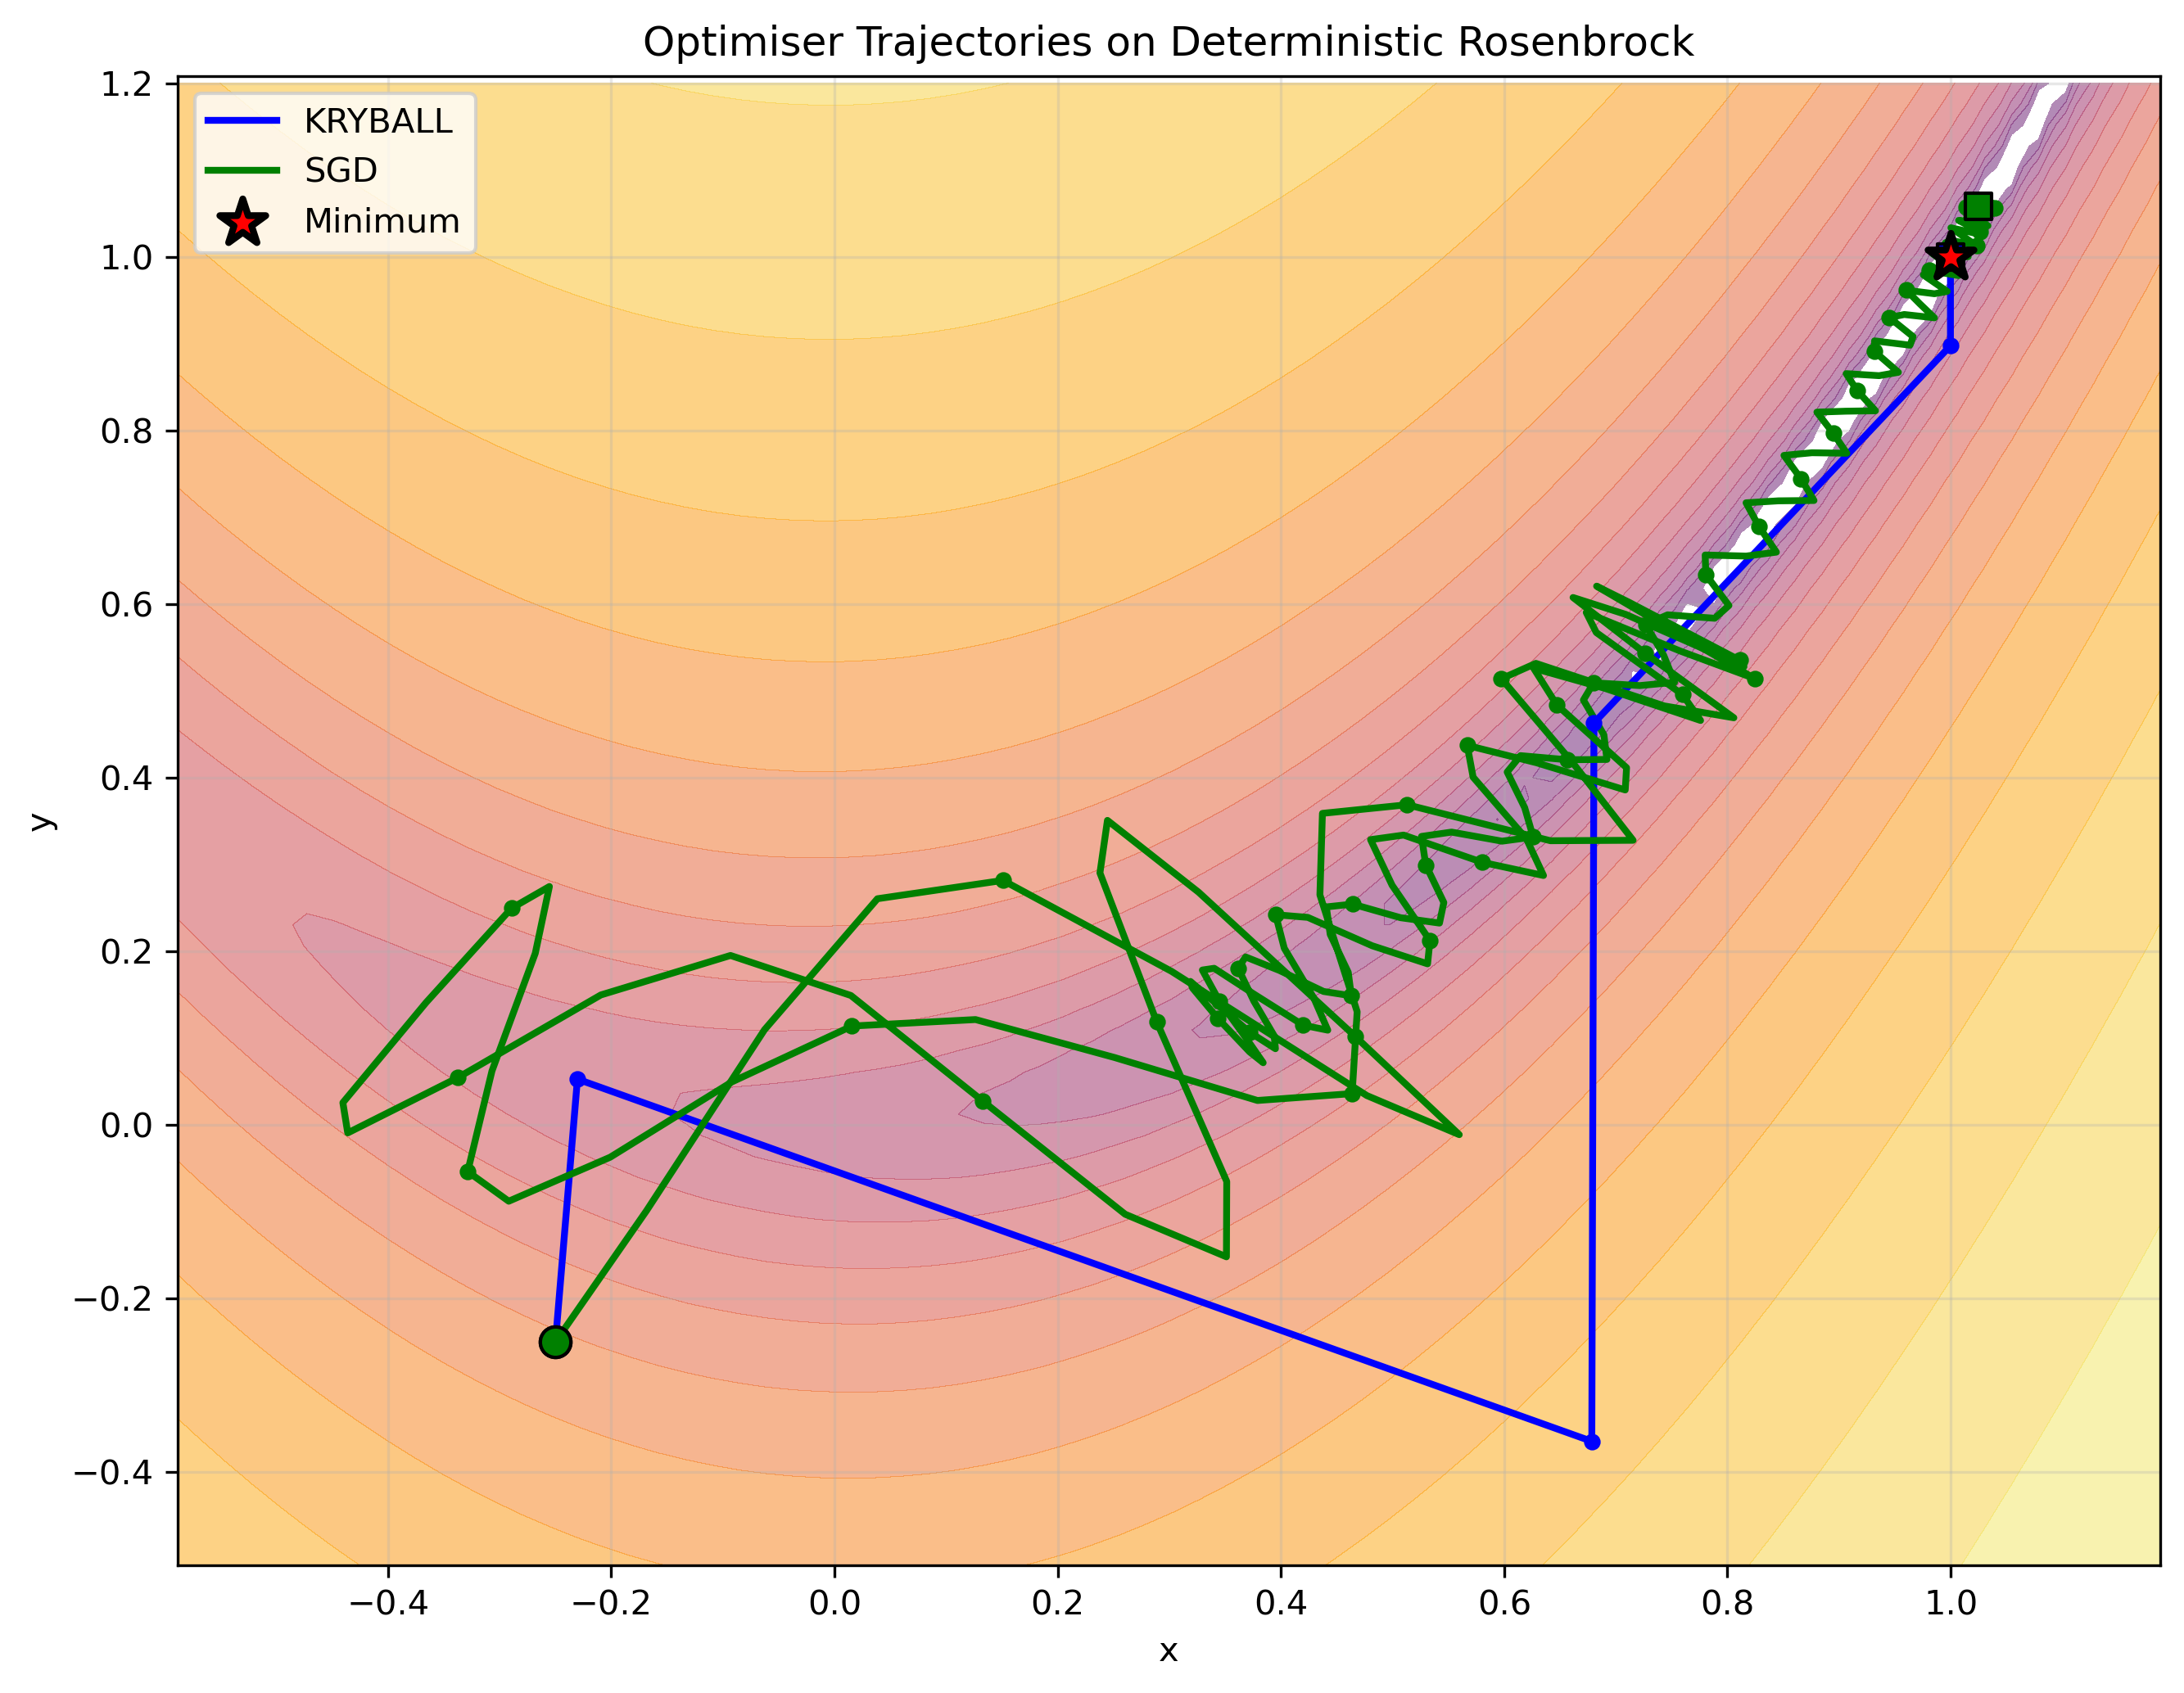
\includegraphics[width=\linewidth]{figures/5evals/deterministic.png}
        \caption{The optimiser trajectories on the deterministic Rosenbrock function with $\lambda_1 = 2$ and $\lambda_2 = 1$.}
        \label{fig:deterministic}
    \end{subfigure}
    \hfill
    \begin{subfigure}[b]{0.49\linewidth}
        \centering
        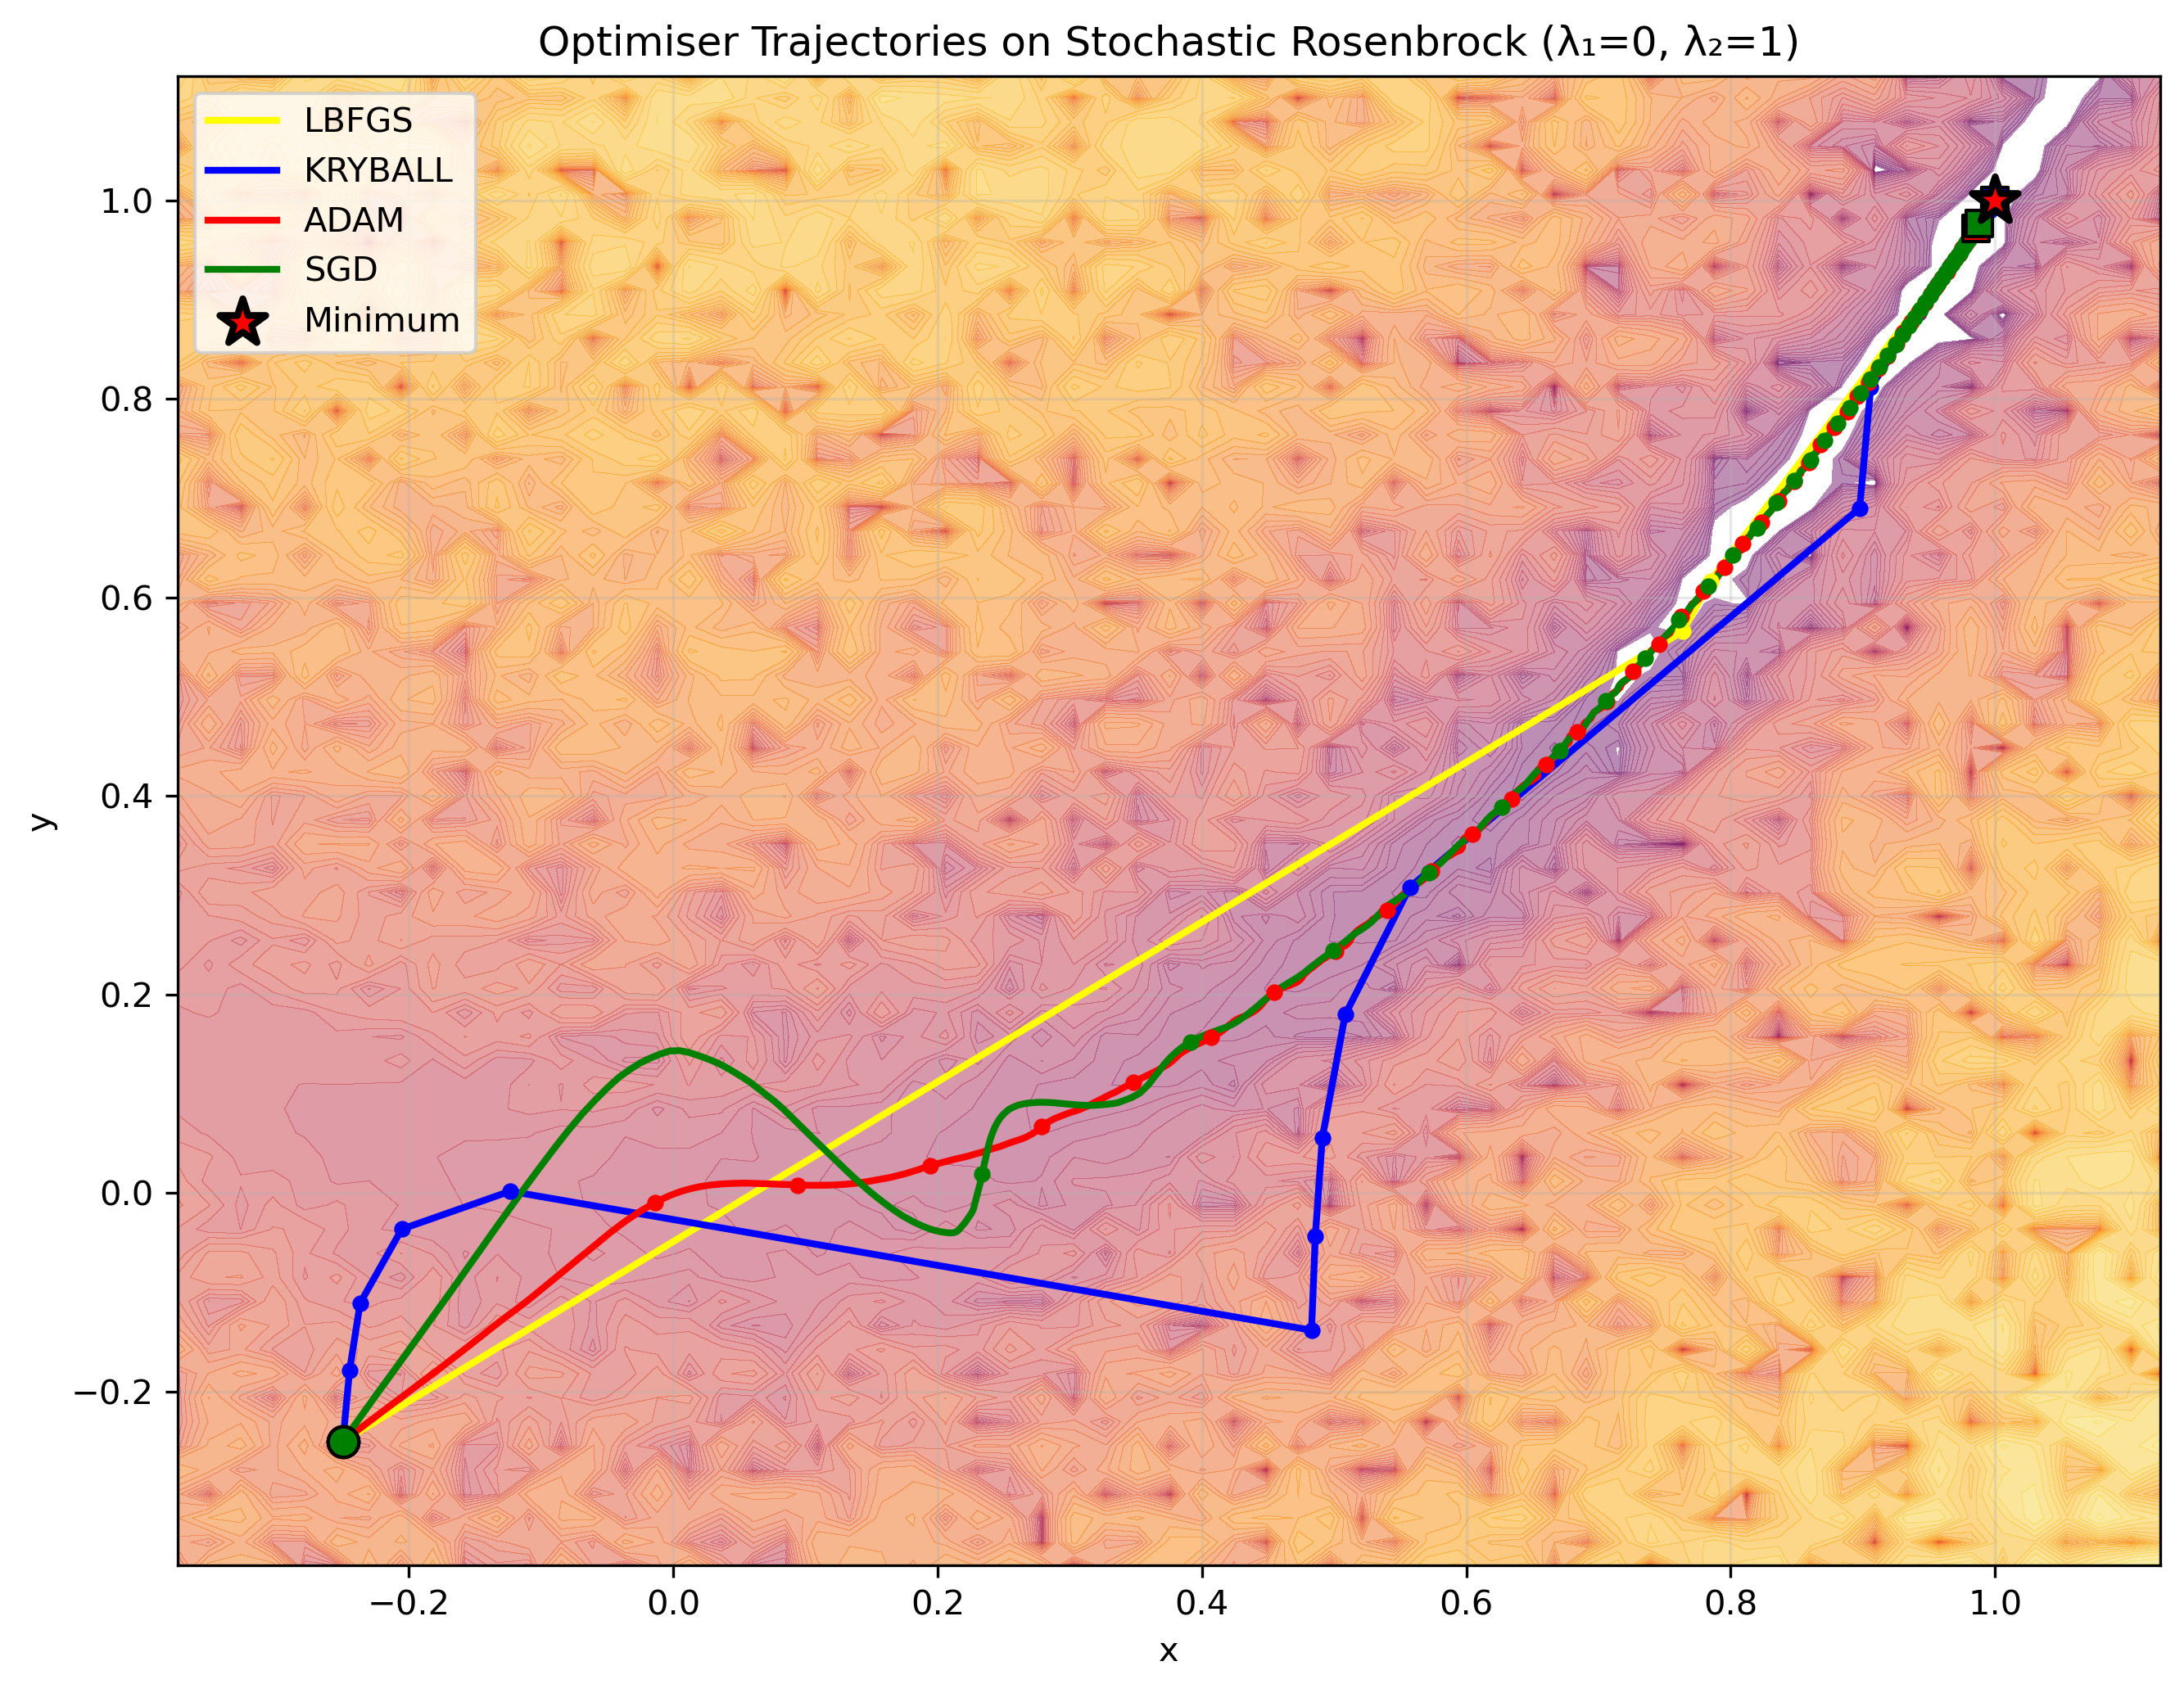
\includegraphics[width=\linewidth]{figures/5evals/stochastic_0_1.png}
        \caption{The optimiser trajectories on the stochastic Rosenbrock function with $\lambda_1 = 0$ and $\lambda_2 = 1$.}
        \label{fig:stochastic_1}
    \end{subfigure}
    
    \vspace{1em}

    \begin{subfigure}[b]{0.49\linewidth}
        \centering
        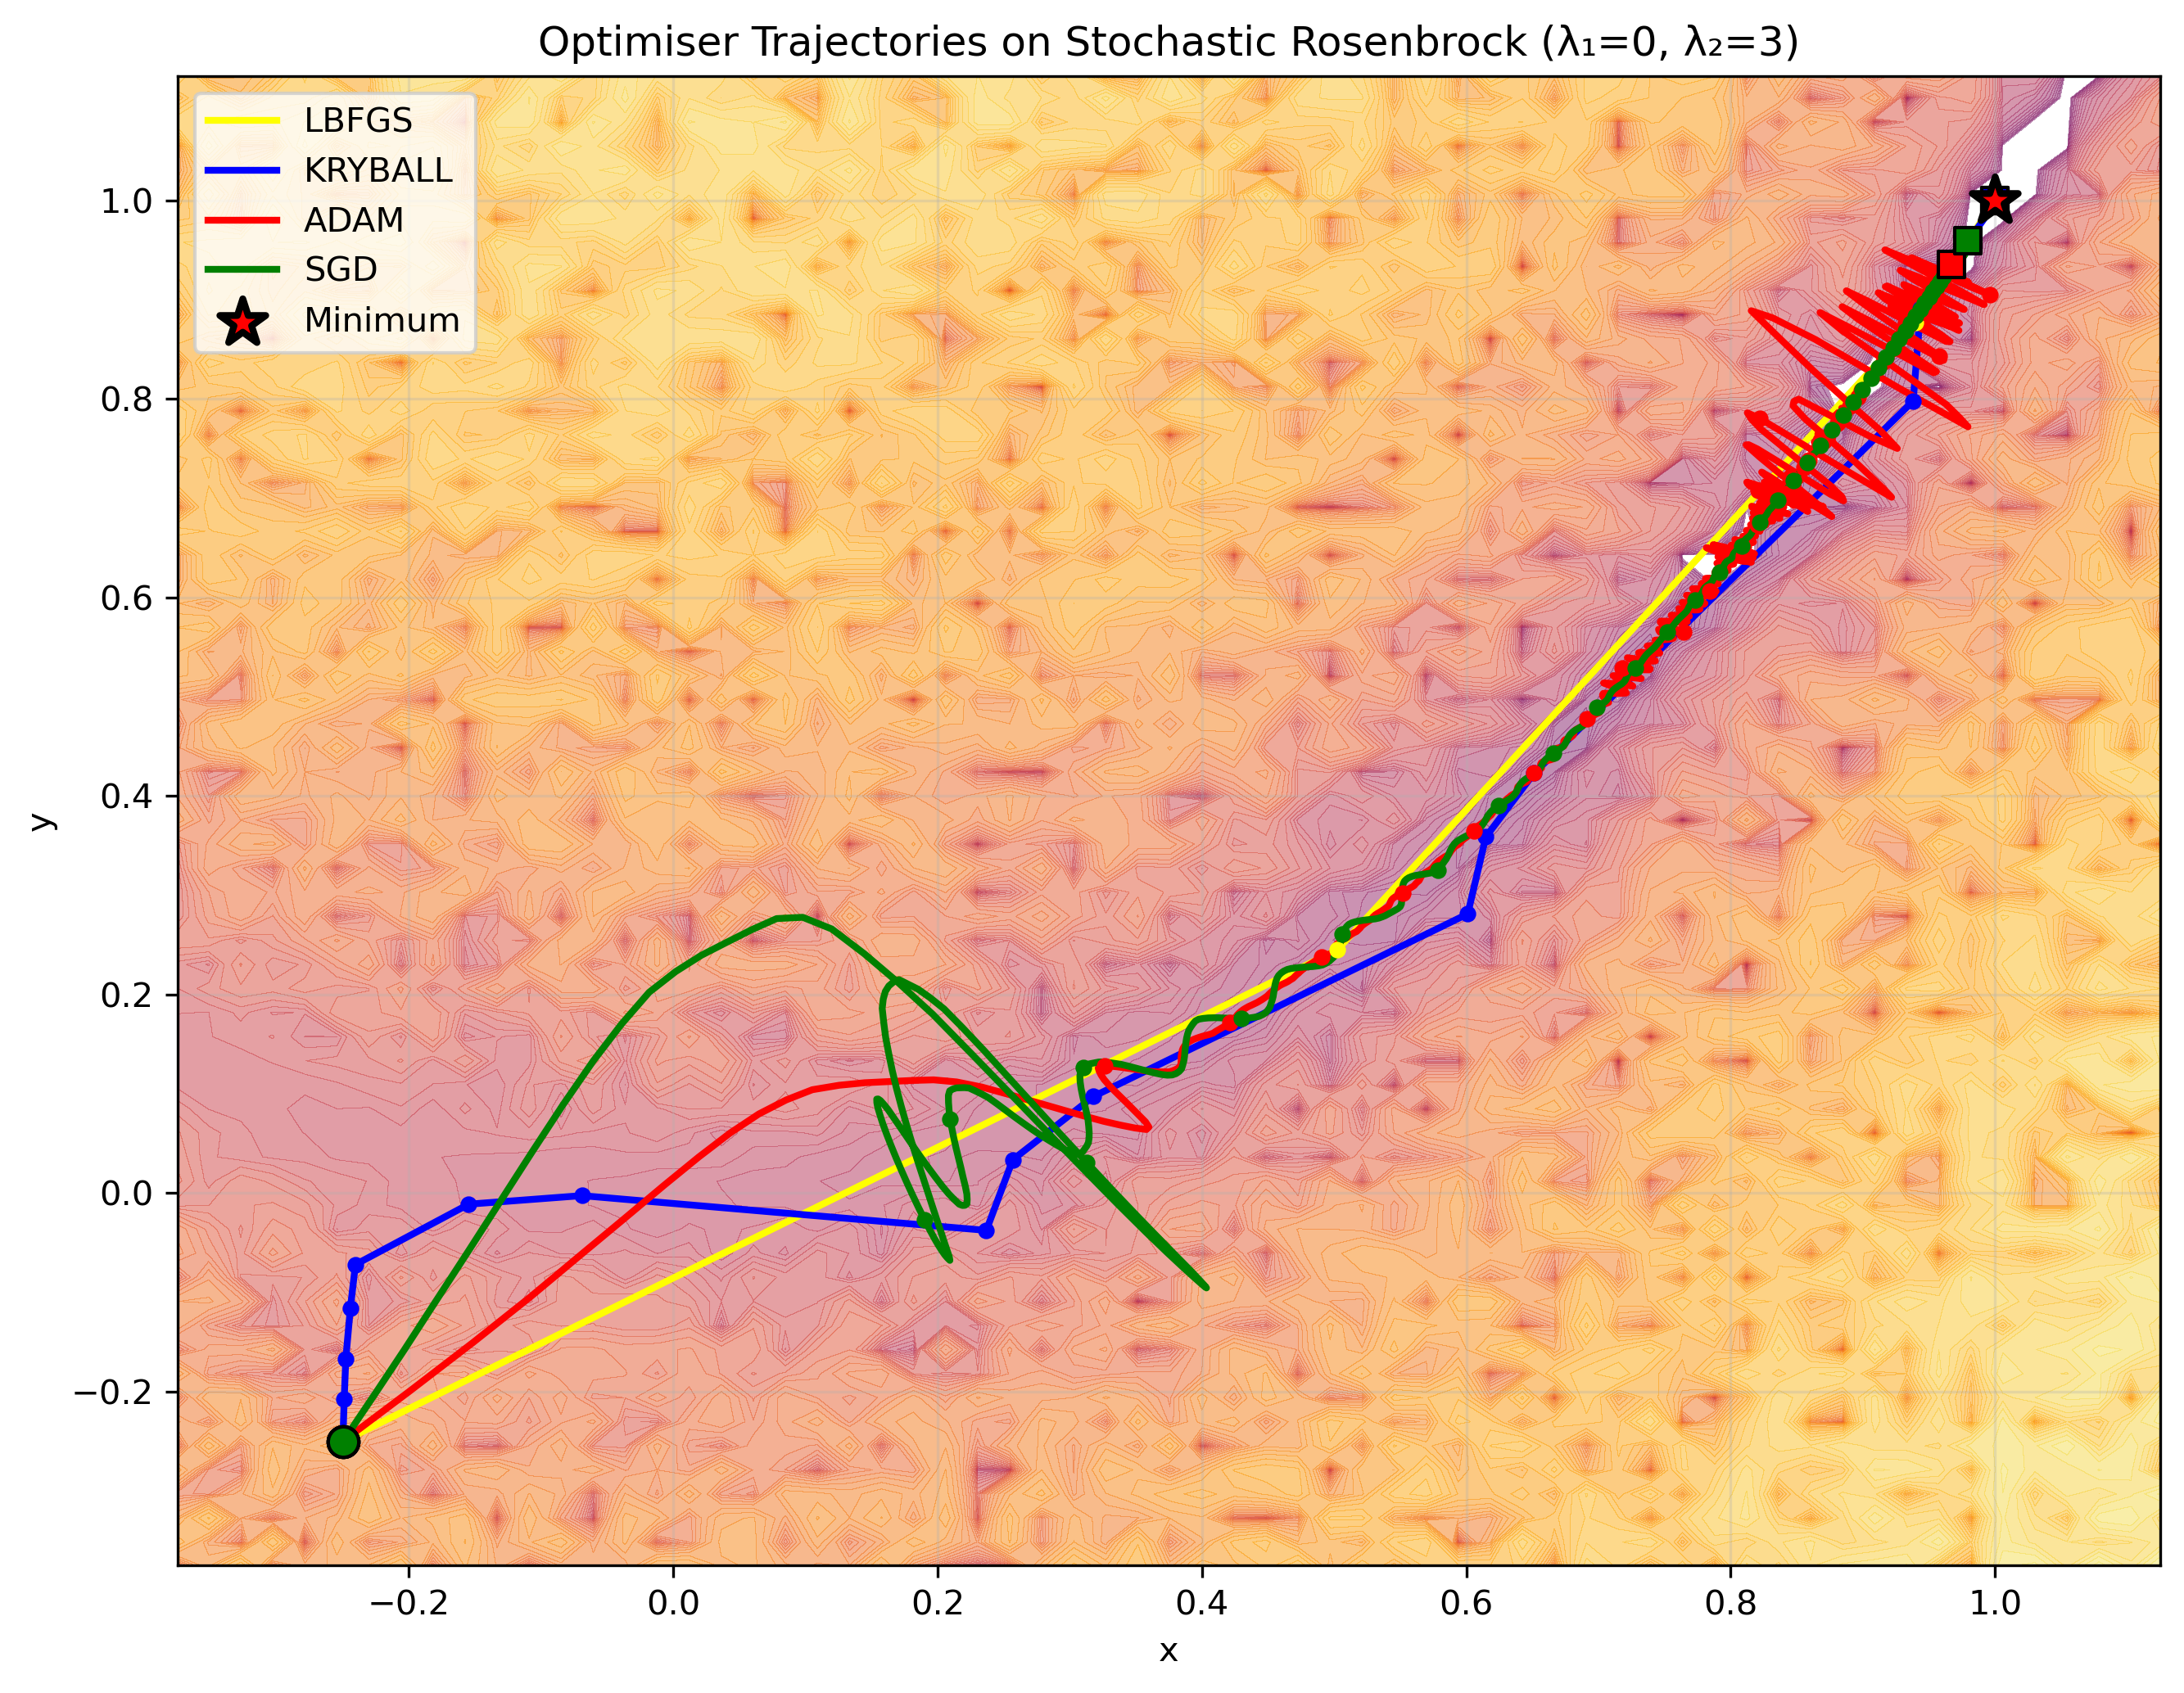
\includegraphics[width=\linewidth]{figures/5evals/stochastic_0_3.png}
        \caption{The optimiser trajectories on the stochastic Rosenbrock function with $\lambda_1 = 0$ and $\lambda_2 = 3$.}
        \label{fig:stochastic_2}
    \end{subfigure}
    \caption{The optimiser trajectories on the deterministic and stochastic Rosenbrock functions. KryBall and LBFGS are able to find the global minimum extremely quickly, and are not impacted by the ill-conditioning of the function. However, MSGD and Adam are impacted and converge much slower to the optimal solution.}
    \label{fig:rosenbrock_results}
\end{figure}

\begin{figure}[!t]
    \begin{subfigure}[b]{0.49\linewidth}
        \centering
        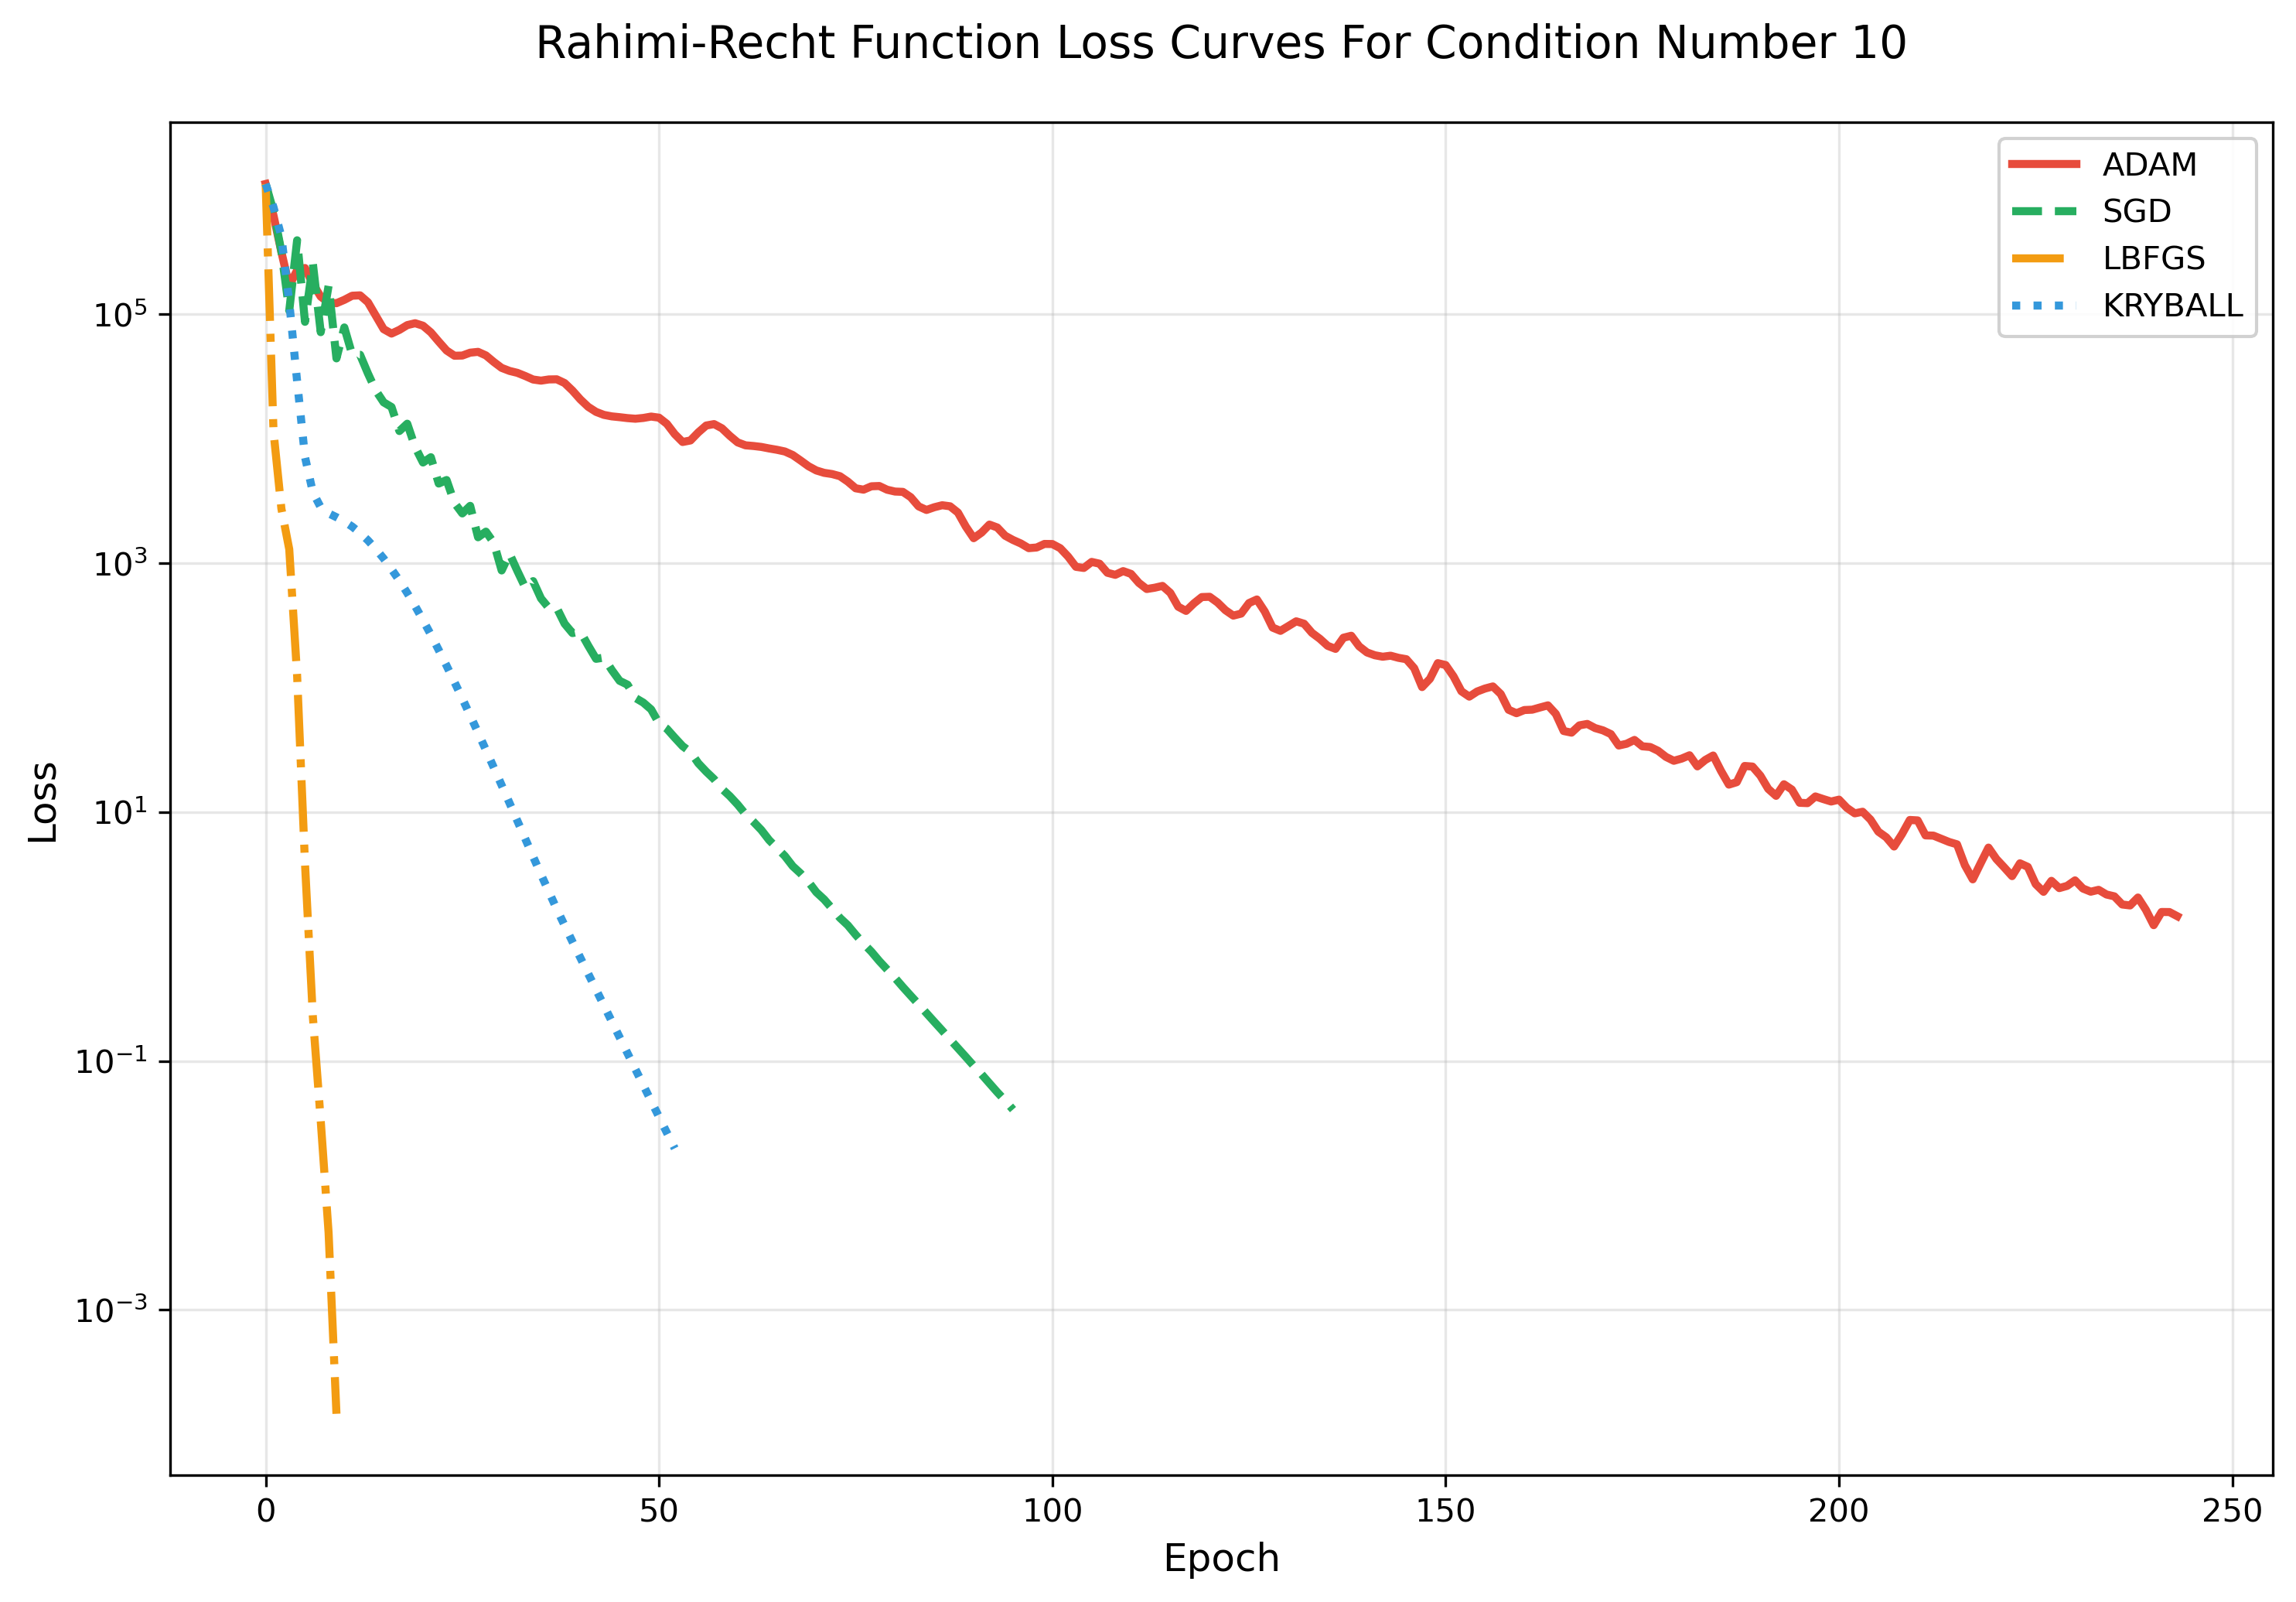
\includegraphics[width=\linewidth]{figures/5evals/rr_losses_k_10.png}
        \caption{Loss curves for the Rahimi-Recht function with condition number $\kappa = 10$.}
        \label{fig:rr_losses_k_10}
    \end{subfigure}
    \hfill
    \begin{subfigure}[b]{0.49\linewidth}
        \centering
        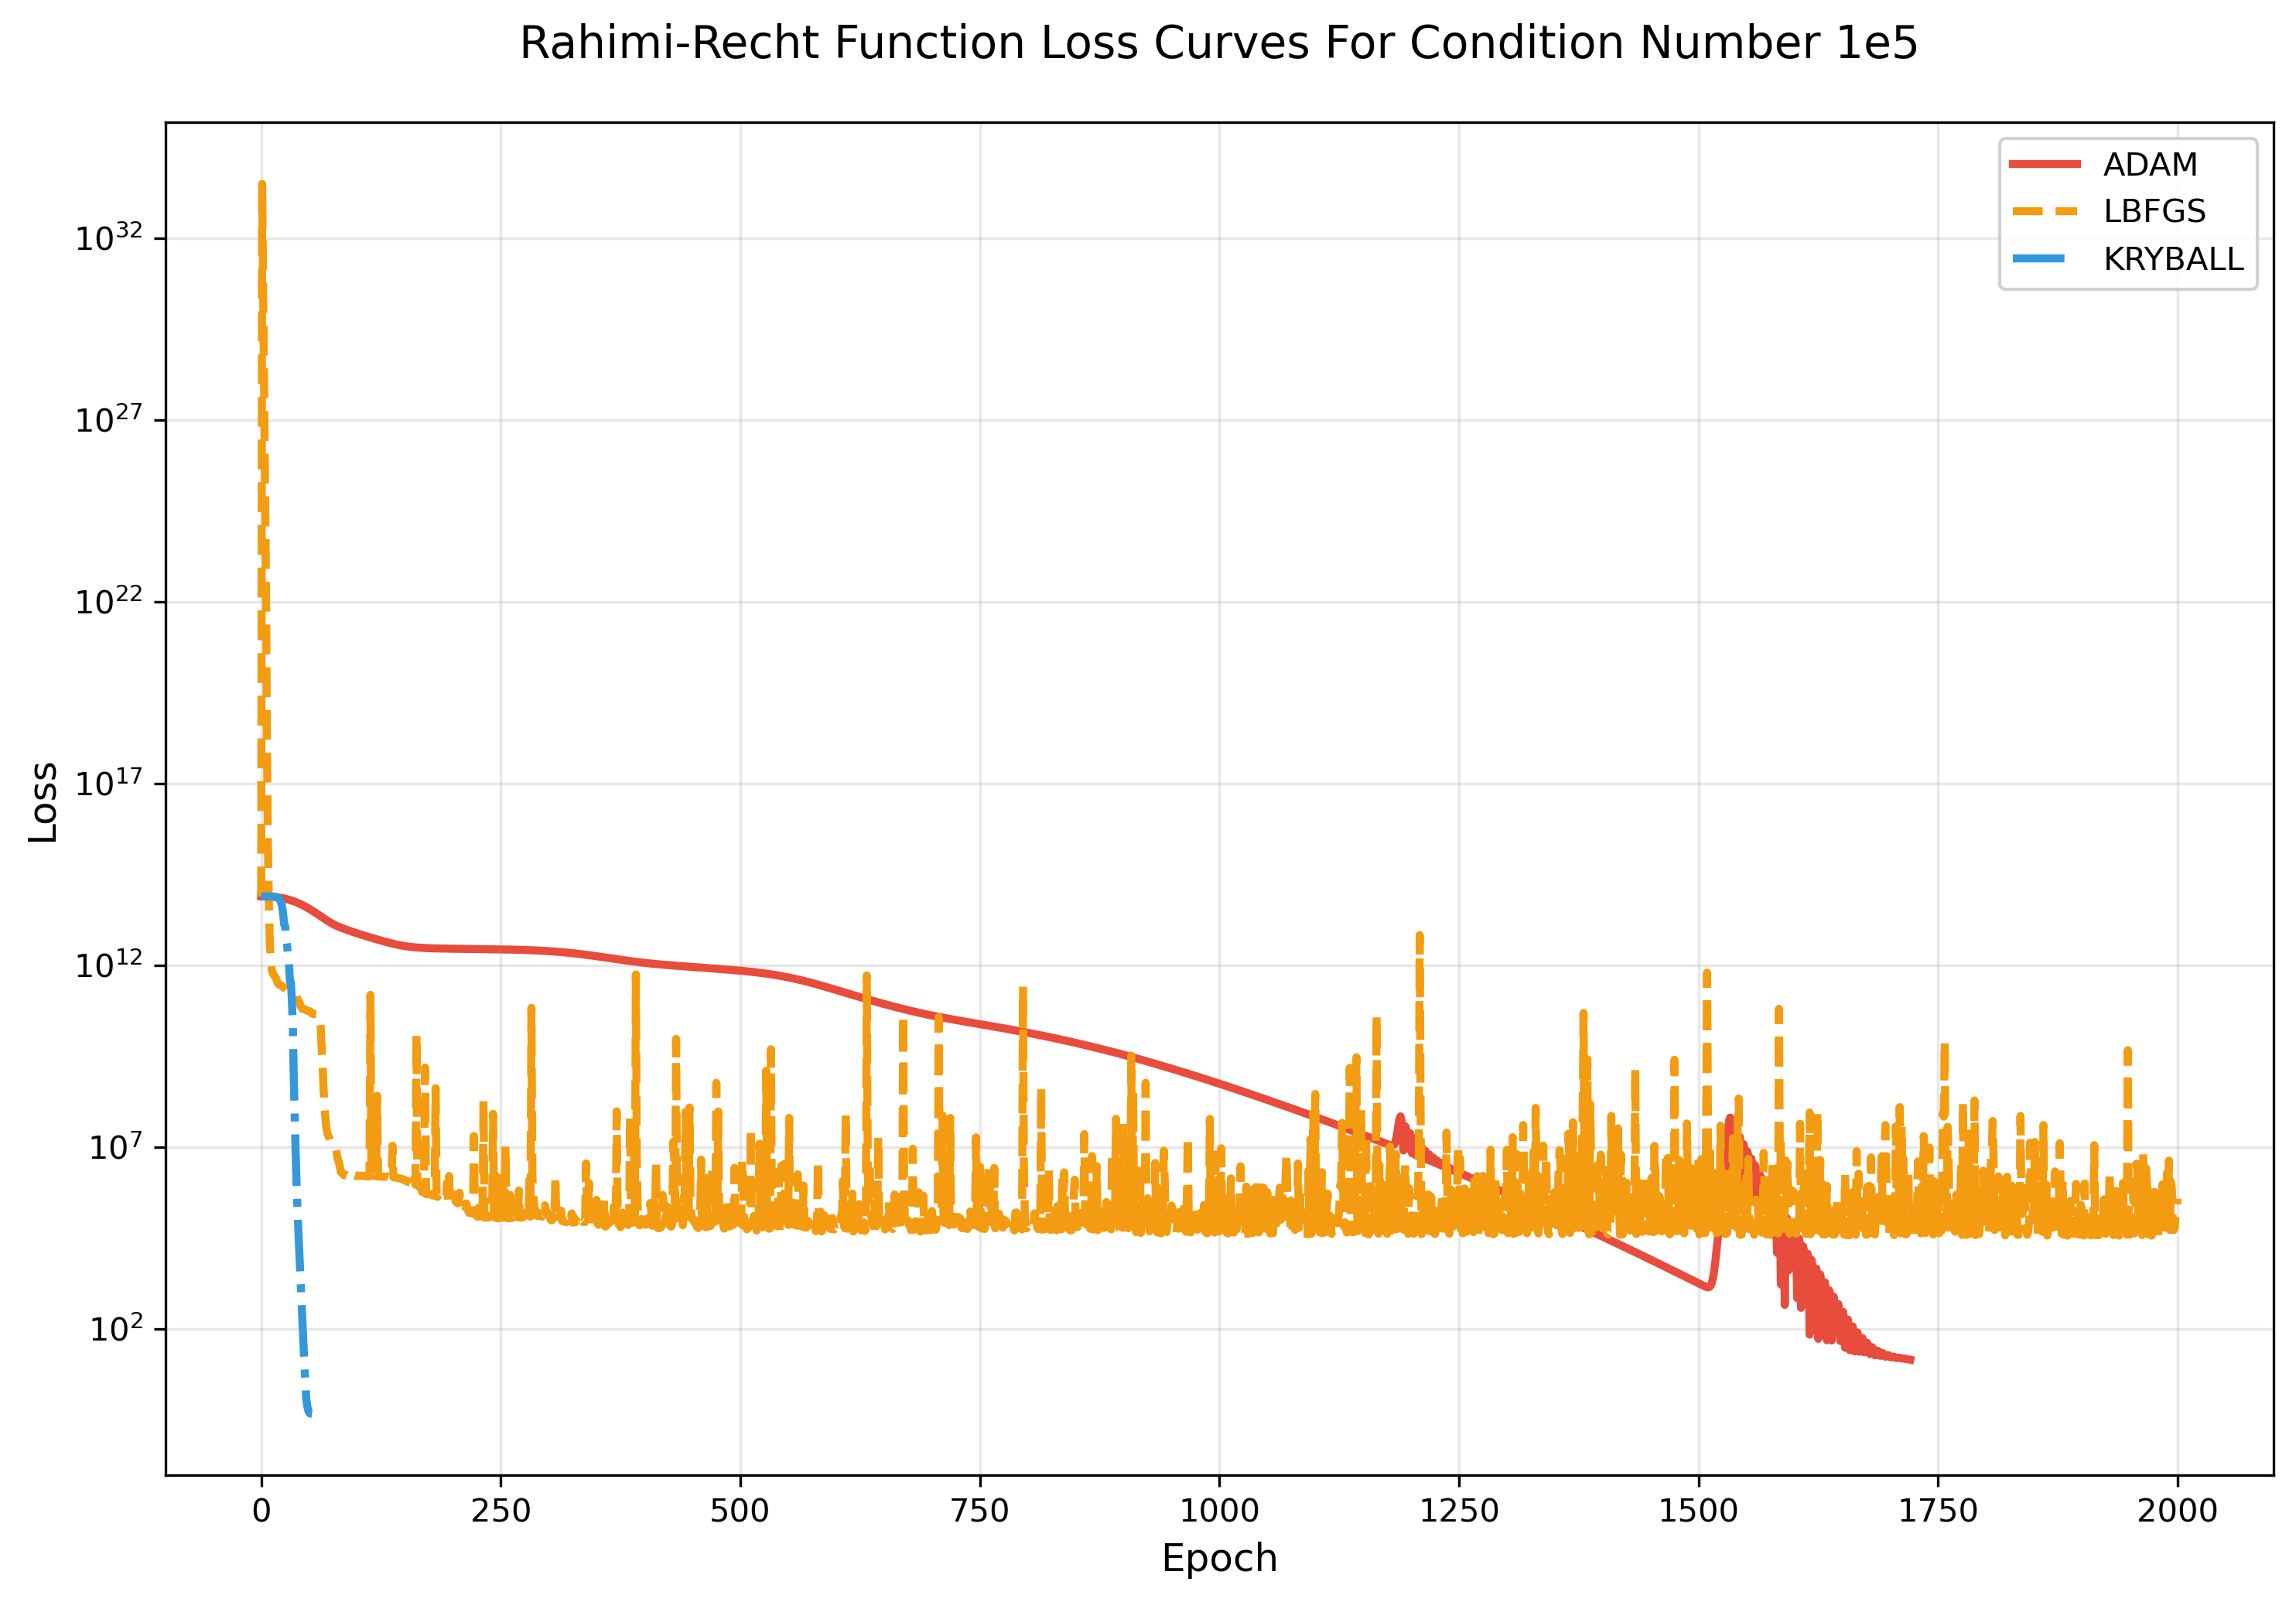
\includegraphics[width=\linewidth]{figures/5evals/rr_losses_k_1e5.png}
        \caption{Loss curves for the Rahimi-Recht function with condition number $\kappa = 1 \times 10^5$.}
        \label{fig:rr_losses_k_1e5}
    \end{subfigure}
    \caption{Loss curves for two instances of the Rahimi-Recht function. In \cref{fig:rr_losses_k_1e5}, we have slight degree of ill-conditioning with $\kappa = 10$, and in \cref{fig:rr_losses_k_10}, we have a very high degree of ill-conditioning with $\kappa = 1 \times 10^5$. We note that in \cref{fig:rr_losses_k_1e5}, MSGD is not here as it diverged in every run very quickly.}
    \label{fig:rr_results}
\end{figure}

\subsection{Task 2: XOR Classification}
\label{ssec:results_xor_classification}

We now move onto our second task, XOR classification. Here, we evaluate the performance of our optimisers based on how quickly the converge to zero loss. We note that here, LBFGS is limited to one evaluation per epoch to make it fair for all optimisers. This is because for many deep learning tasks, we no longer have a best case pratical scenario or upper bound and need to ensure a fair comparison.

\begin{figure}[!t]
    \centering
    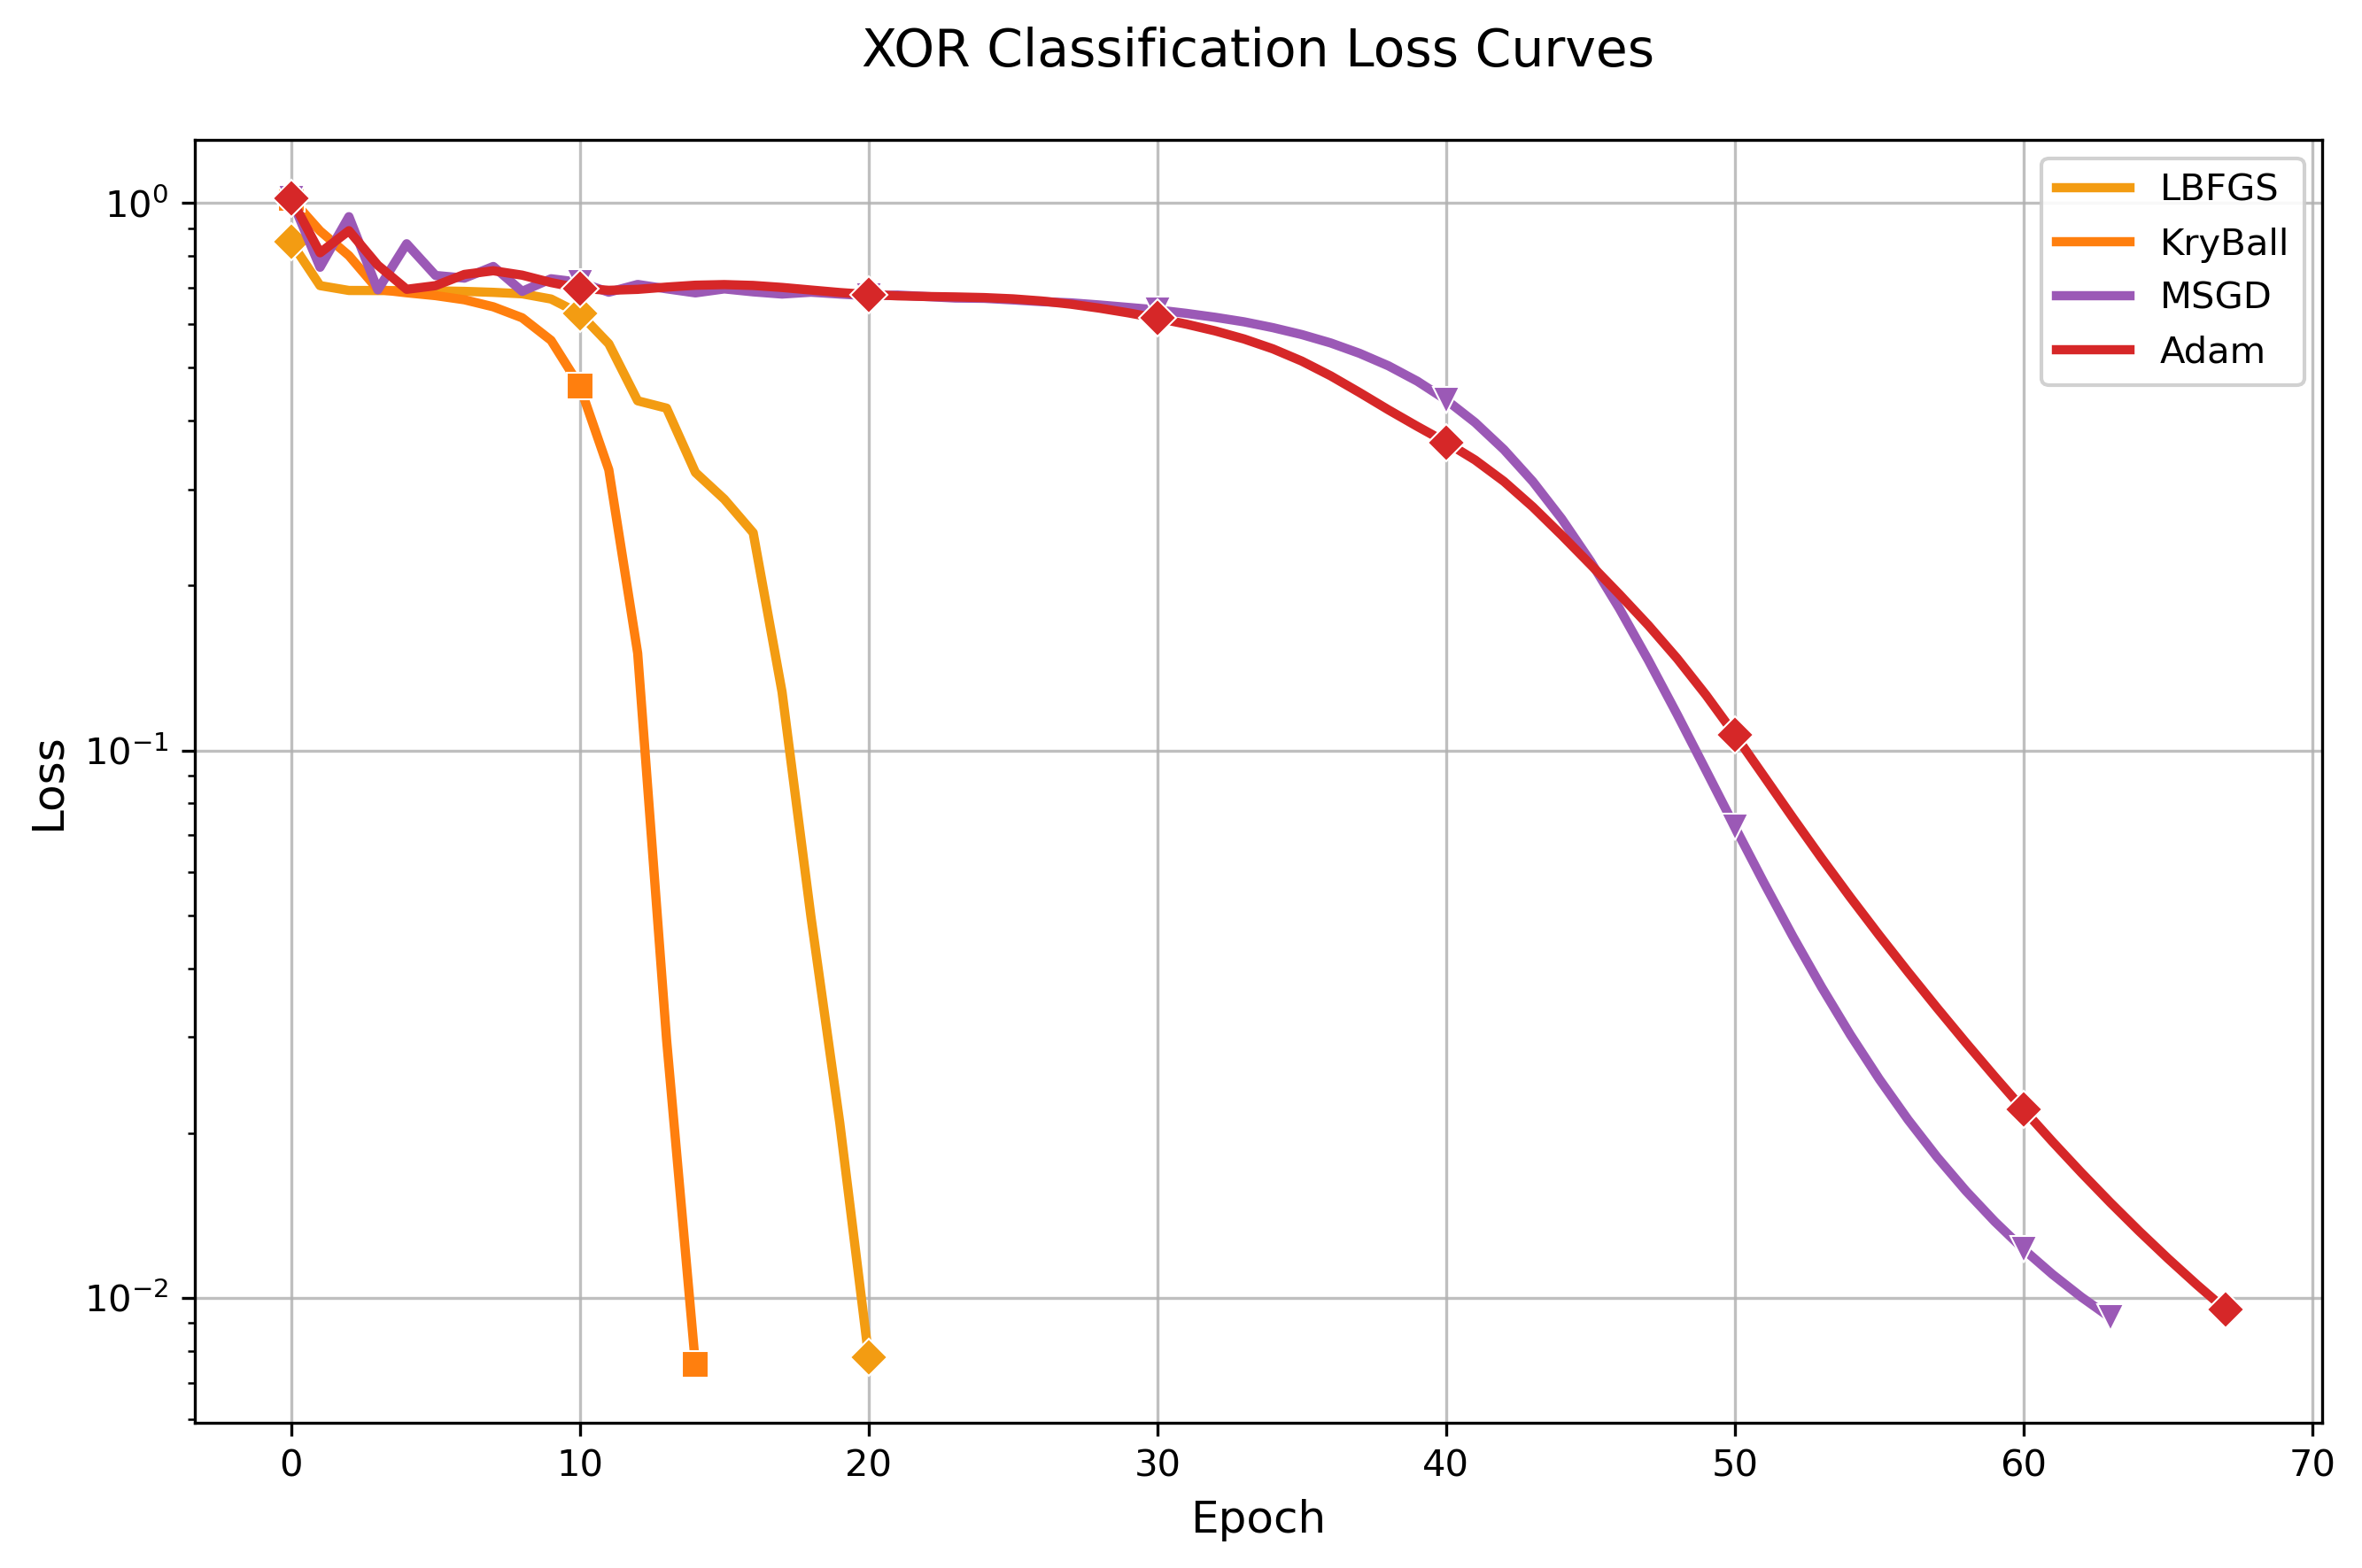
\includegraphics[width=0.6\linewidth]{figures/5evals/xor_losses.png}
    \caption{The loss curves for the XOR classification task. KryBall converges in 15 epochs, MSGD converges in 63 epochs and Adam converges to 67 epochs. LBFGS restricted to one evaluation per iteration converges in 20 epochs.}
    \label{fig:xor_results}
\end{figure}

\cref{fig:xor_results} shows the loss curves. We see that KryBall and LBFGS converge the quickest, in less than 25 epochs. MSGD and Adam are also able to converge, but take longer. This shows that KryBall is able to generalise very quickly, and that the second-order approximation is helpful in identifying the optimal solution. As such, this shows in the simplest setting that our approximation is useful in tasks where there are non-linearities involved. As we now transition into harder tasks that are highly parameterised and likely non-linear, we hypothesise that our quadratic model will be able to generalise and add more insight into the optimisation landscape.

We note that while this task is simple and may seem trivial, it is a good baseline and a bridge to more complex tasks in the next section. We now move onto these tasks in the next section.

\subsection{Task 3: Image Classification}
\label{ssec:results_image_classification}

We now move into the primary focus of our results, evaluating our optimiser on standard deep-learning tasks that are the benchmark for optimisers. We evaluate our optimisers on three image classification tasks: MNIST-1D, CIFAR-10 CNN, and CIFAR-10 ResNet-18, which we described in \cref{ssec:task_3_image_classification}. We note that from here onwards, we do not use LBFGS since it becomes too expensive and compute heavy to evaluate. Thus, our optimiser suite is now Adam, MSGD and KryBall. We present a summary of our results in \Cref{tab:classification_results}. Our loss curves and accuracies are provided in \cref{fig:image_classification_results}. 

% Please add the following required packages to your document preamble:
% \usepackage{multirow}
% \usepackage[table,xcdraw]{xcolor}
% Beamer presentation requires \usepackage{colortbl} instead of \usepackage[table,xcdraw]{xcolor}
\begin{table}[!t]
    \centering
    \caption{Classification results for MNIST1D MLP, CIFAR10 CNN, and CIFAR10 ResNet-18 given Adam, MSGD and KryBall optimisers.}
    \label{tab:classification_results}
    \begin{tabular}{ccccc}
    \hline
                                                                                            & \textbf{Method} & \textbf{\begin{tabular}[c]{@{}c@{}}Final \\ Training \\ Loss $\downarrow$\end{tabular}} & \textbf{\begin{tabular}[c]{@{}c@{}}Peak \\ Test\\ Accuracy $\uparrow$\end{tabular}} & \textbf{\begin{tabular}[c]{@{}c@{}}Final \\ Test\\ Accuracy $\uparrow$\end{tabular}} \\ \hline
                                                                                            & Adam            & \cellcolor[HTML]{FFFFFF}0.144                                              & \cellcolor[HTML]{FFFFFF}0.668                                            & \cellcolor[HTML]{FFFFFF}0.668                                             \\
                                                                                            & MSGD            & \cellcolor[HTML]{FFFFFF}0.326                                              & \cellcolor[HTML]{FFFFFF}0.669                                            & \cellcolor[HTML]{FFFFFF}0.644                                             \\
    \multirow{-3}{*}{\textbf{\begin{tabular}[c]{@{}c@{}}MNIST1D\\ MLP\end{tabular}}}        & KryBall         & \cellcolor[HTML]{34FF34}\textbf{0.001}                                     & \cellcolor[HTML]{34FF34}\textbf{0.685}                                   & \cellcolor[HTML]{34FF34}\textbf{0.685}                                    \\ \hline
                                                                                            & Adam            & \cellcolor[HTML]{34FF34}\textbf{0.099}                                     & 0.782                                                                    & \cellcolor[HTML]{34FF34}\textbf{0.777}                                    \\
                                                                                            & MSGD            & 0.111                                                                      & 0.777                                                                    & 0.771                                                                     \\
    \multirow{-3}{*}{\textbf{\begin{tabular}[c]{@{}c@{}}CIFAR10 \\ CNN\end{tabular}}}       & KryBall         & 0.135                                                                      & \cellcolor[HTML]{34FF34}\textbf{0.783}                                   & 0.762                                                                     \\ \hline
                                                                                            & Adam            & \cellcolor[HTML]{34FF34}\textbf{7.5e-5}                                    & \cellcolor[HTML]{34FF34}\textbf{0.843}                                   & \cellcolor[HTML]{34FF34}\textbf{0.842}                                    \\
                                                                                            & MSGD            & 1e-4                                                                       & 0.832                                                                    & 0.829                                                                     \\
    \multirow{-3}{*}{\textbf{\begin{tabular}[c]{@{}c@{}}CIFAR10 \\ ResNet-18\end{tabular}}} & KryBall         & 0.002                                                                      & 0.832                                                                    & 0.822                                                                     \\ \hline
    \end{tabular}
    \end{table}

\begin{figure}[!t]
    \centering
    % First column
    \begin{subfigure}[b]{0.48\linewidth}  % Wider subfigures (0.48 instead of 0.32)
        \centering
        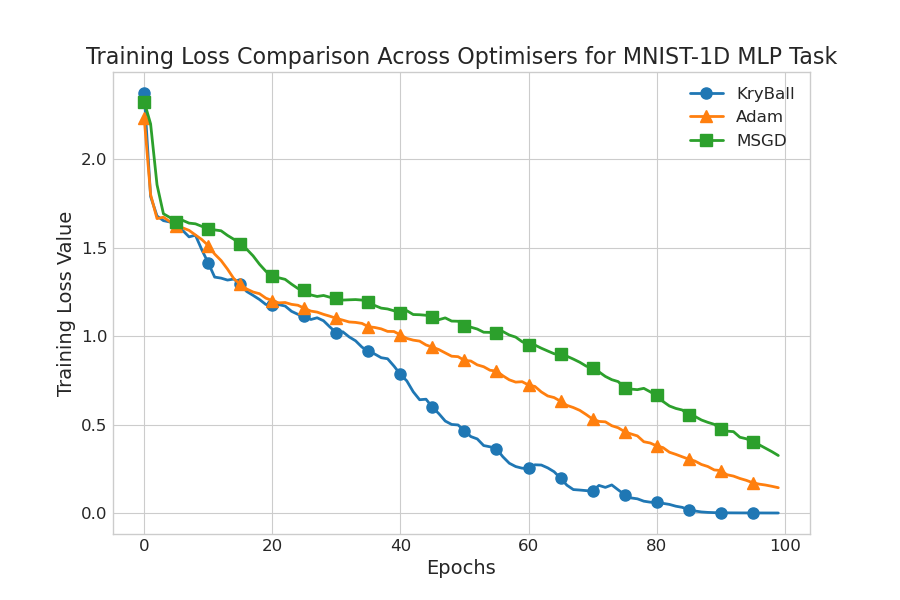
\includegraphics[width=\linewidth]{figures/5evals/mnist1d_mlp_loss.png}
        \caption{Training Loss on MNIST-1D MLP}
        \label{fig:mnist1d_mlp_loss}
    \end{subfigure}
    \begin{subfigure}[b]{0.48\linewidth}
        \centering
        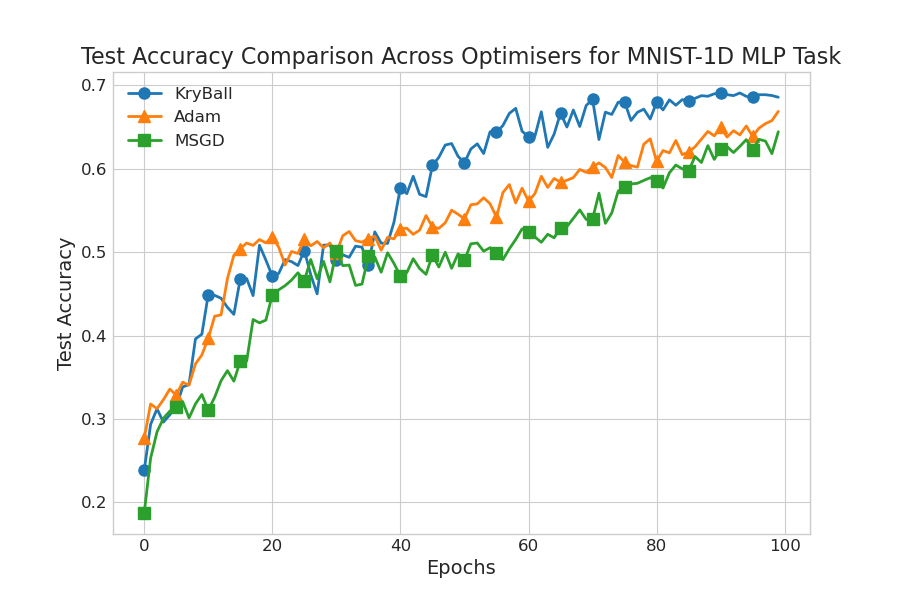
\includegraphics[width=\linewidth]{figures/5evals/mnist1d_mlp_acc.png}
        \caption{Training Accuracy on MNIST-1D MLP}
        \label{fig:mnist1d_mlp_acc}
    \end{subfigure}
    
    \vspace{1em}  % Add vertical space between rows
    
    % Second row
    \begin{subfigure}[b]{0.45\linewidth}
        \centering
        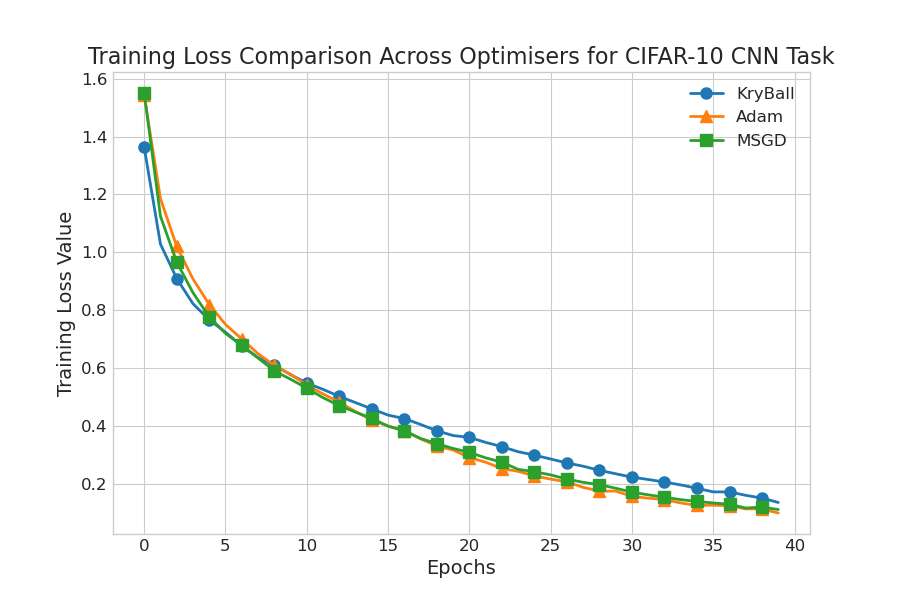
\includegraphics[width=\linewidth]{figures/5evals/cifar10_cnn_loss.png}
        \caption{Training Loss on CIFAR-10 CNN}
        \label{fig:cifar10_cnn_loss}
    \end{subfigure}
    \hfill
    \begin{subfigure}[b]{0.48\linewidth}
        \centering
        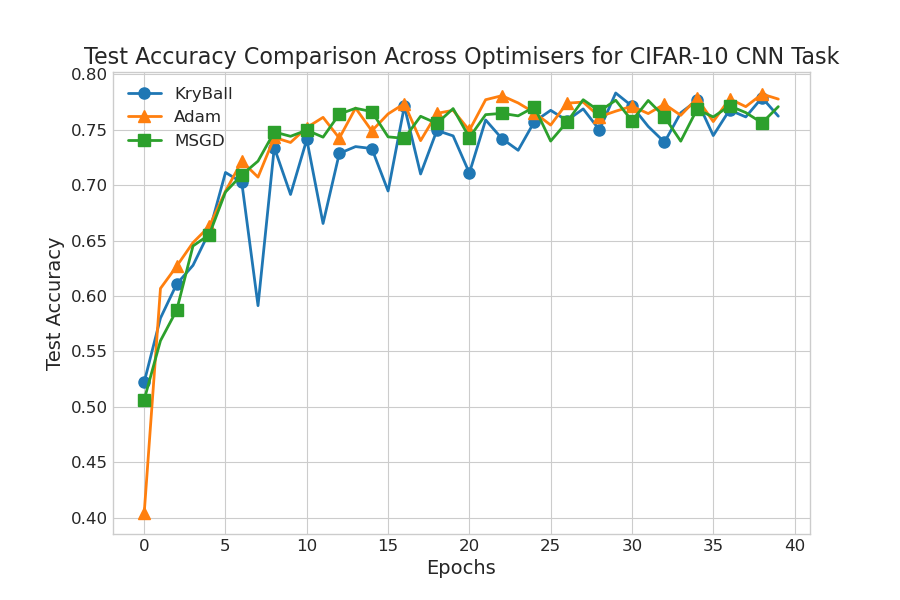
\includegraphics[width=\linewidth]{figures/5evals/cifar10_cnn_acc.png}
        \caption{Training Accuracy on CIFAR-10 CNN}
        \label{fig:cifar10_cnn_acc}
    \end{subfigure}
    
    \vspace{1em}  % Add vertical space between rows
    
    % Third row
    \begin{subfigure}[b]{0.48\linewidth}
        \centering
        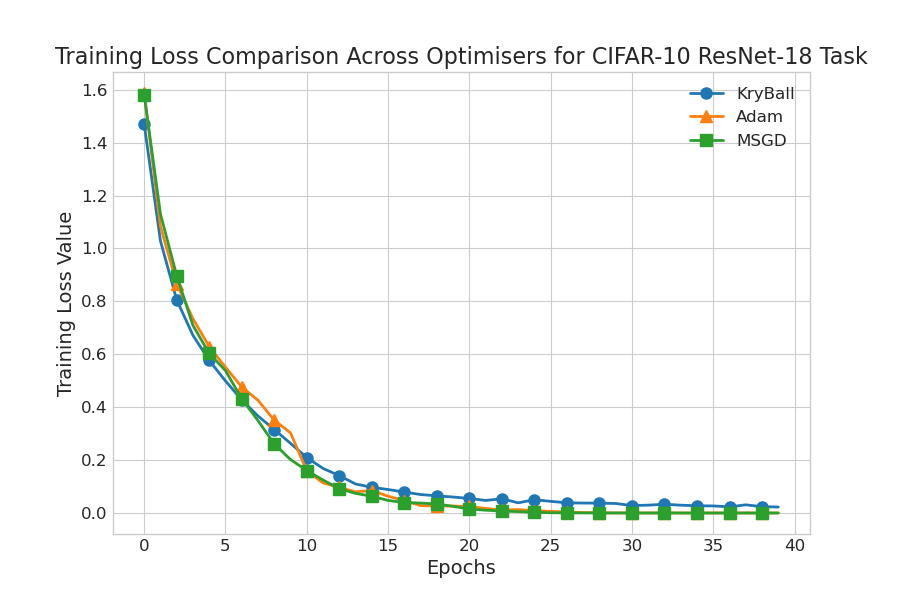
\includegraphics[width=\linewidth]{figures/5evals/cifar10_resnet_loss.png}  % Replace with actual duplicate figure
        \caption{Training Loss on CIFAR-10 ResNet-18}
        \label{fig:cifar10_resnet_loss}
    \end{subfigure}
    \hfill
    \begin{subfigure}[b]{0.48\linewidth}
        \centering
        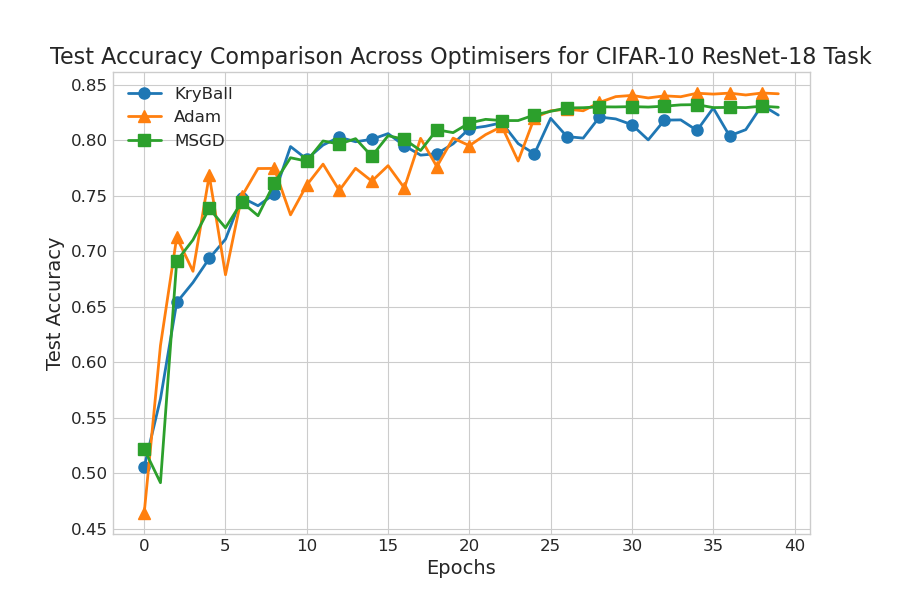
\includegraphics[width=\linewidth]{figures/5evals/cifar10_resnet_acc.png}  % Replace with actual duplicate figure
        \caption{Training Accuracy on CIFAR-10 ResNet-18}
        \label{fig:cifar10_resnet_acc}
    \end{subfigure}
    
    \caption{Loss curves and test accuracy comparisons among our image classification tasks consisting of MNIST-1D MLP, CIFAR-10 CNN and CIFAR-10 ResNet-18. Each task is evaluated with KryBall, Adam and MSGD.}
    \label{fig:image_classification_results}
\end{figure}

\textbf{MNIST-1D MLP}: KryBall demonstrates a clear advantage for the MNIST-1D MLP task. It is able to achieve the highest peak accuracy and the lowest final training loss. \cref{fig:mnist1d_mlp_loss} and \cref{fig:mnist1d_mlp_acc} show that KryBall converges quickly and makes a large improvement over Adam and MSGD, especially in 40 to 80 epoch range. We note that while a peak accuracy of 0.685 may not sound high, this contends with the best result on this specific model for MNIST-1D \cite{greydanus_mnist1d}. As such, we outperform Adam and MSGD in all metrics.

\textbf{CIFAR-10 CNN}: Here, we see a more nuanced performance. Adam achieves the lowest final training loss, alongside the best final test accuracy. However, KryBall slightly outperforms Adam and records a higher peak test accuracy. The training loss curves in \cref{fig:cifar10_cnn_loss} show Adam and MSGD reaching a slightly lower loss plateau than KryBall. In terms of test accuracy curves in \cref{fig:cifar10_cnn_acc}, all three optimisers are competitive, with KryBall showing a strong peak but Adam and MSGD achieve slightly better peak test accuracy. A key observation here is that in \cref{fig:cifar10_cnn_acc}, KryBall originally has a lower training loss, but then is surpassed by Adam and MSGD as training continue. During epochs 10 to 25, KryBall is also quite variant before converging. This is unlike Adam and MSGD, who are consistent all the way. 

\textbf{CIFAR-10 ResNet-18}: We see a similar comparison here. Adam has the best final training loss, and best peak test and final test accuracy. However, KryBall is generally competitive with Adam and MSGD. It achieves the same best test accuracy as MSGD, and only a slightly lower final test accuracy. Furthermore, \cref{fig:cifar10_resnet_loss} shows the same trend as in \cref{fig:cifar10_cnn_loss}, where KryBall is initially competitive and achieves a lower training loss, but then is surpassed by Adam and MSGD as training continues. In \cref{fig:cifar10_resnet_acc}, we see that KryBall is more stable than Adam and MSGD in the earlier epochs, but less stable in the later epochs and thus its performance suffers. The late epoch instability is also seen in \cref{fig:cifar10_cnn_acc}. 

To recap, KryBall outperforms the state-of-the art Adam and MSGD on the MNIST-1D MLP task, but does not outperform them on the CIFAR-10 tasks. More interestingly, we see that KryBall achieves lower training loss initially in all tasks early on, but then is surpassed by Adam and MSGD as training continues for the CIFAR-10 tasks. Near the end of training, KryBall is less stable than Adam and MSGD and is more variant. We discuss this further in\cref{sec:discussion_and_further_analysis}.

\subsection{Sensitivity Analysis}
\label{ssec:sensitivity_analysis}

We now perform a sensitivity analysis of our method on the MNIST-1D MLP task. We choose this since it is our best performing task. Our sensitive analysis is on the Krylov subspace dimension $M$ and the krylov refresh rate $r_{\mathit{refresh}}$. This is done by varying $M$ and $r_{\mathit{refresh}}$ from their hyperparameter ranges and keeping all other hyperparameters constant. We present the results in \cref{fig:sensitivity_analysis}.

\begin{figure}[!t]
    \begin{subfigure}[b]{0.49\linewidth}
        \centering
        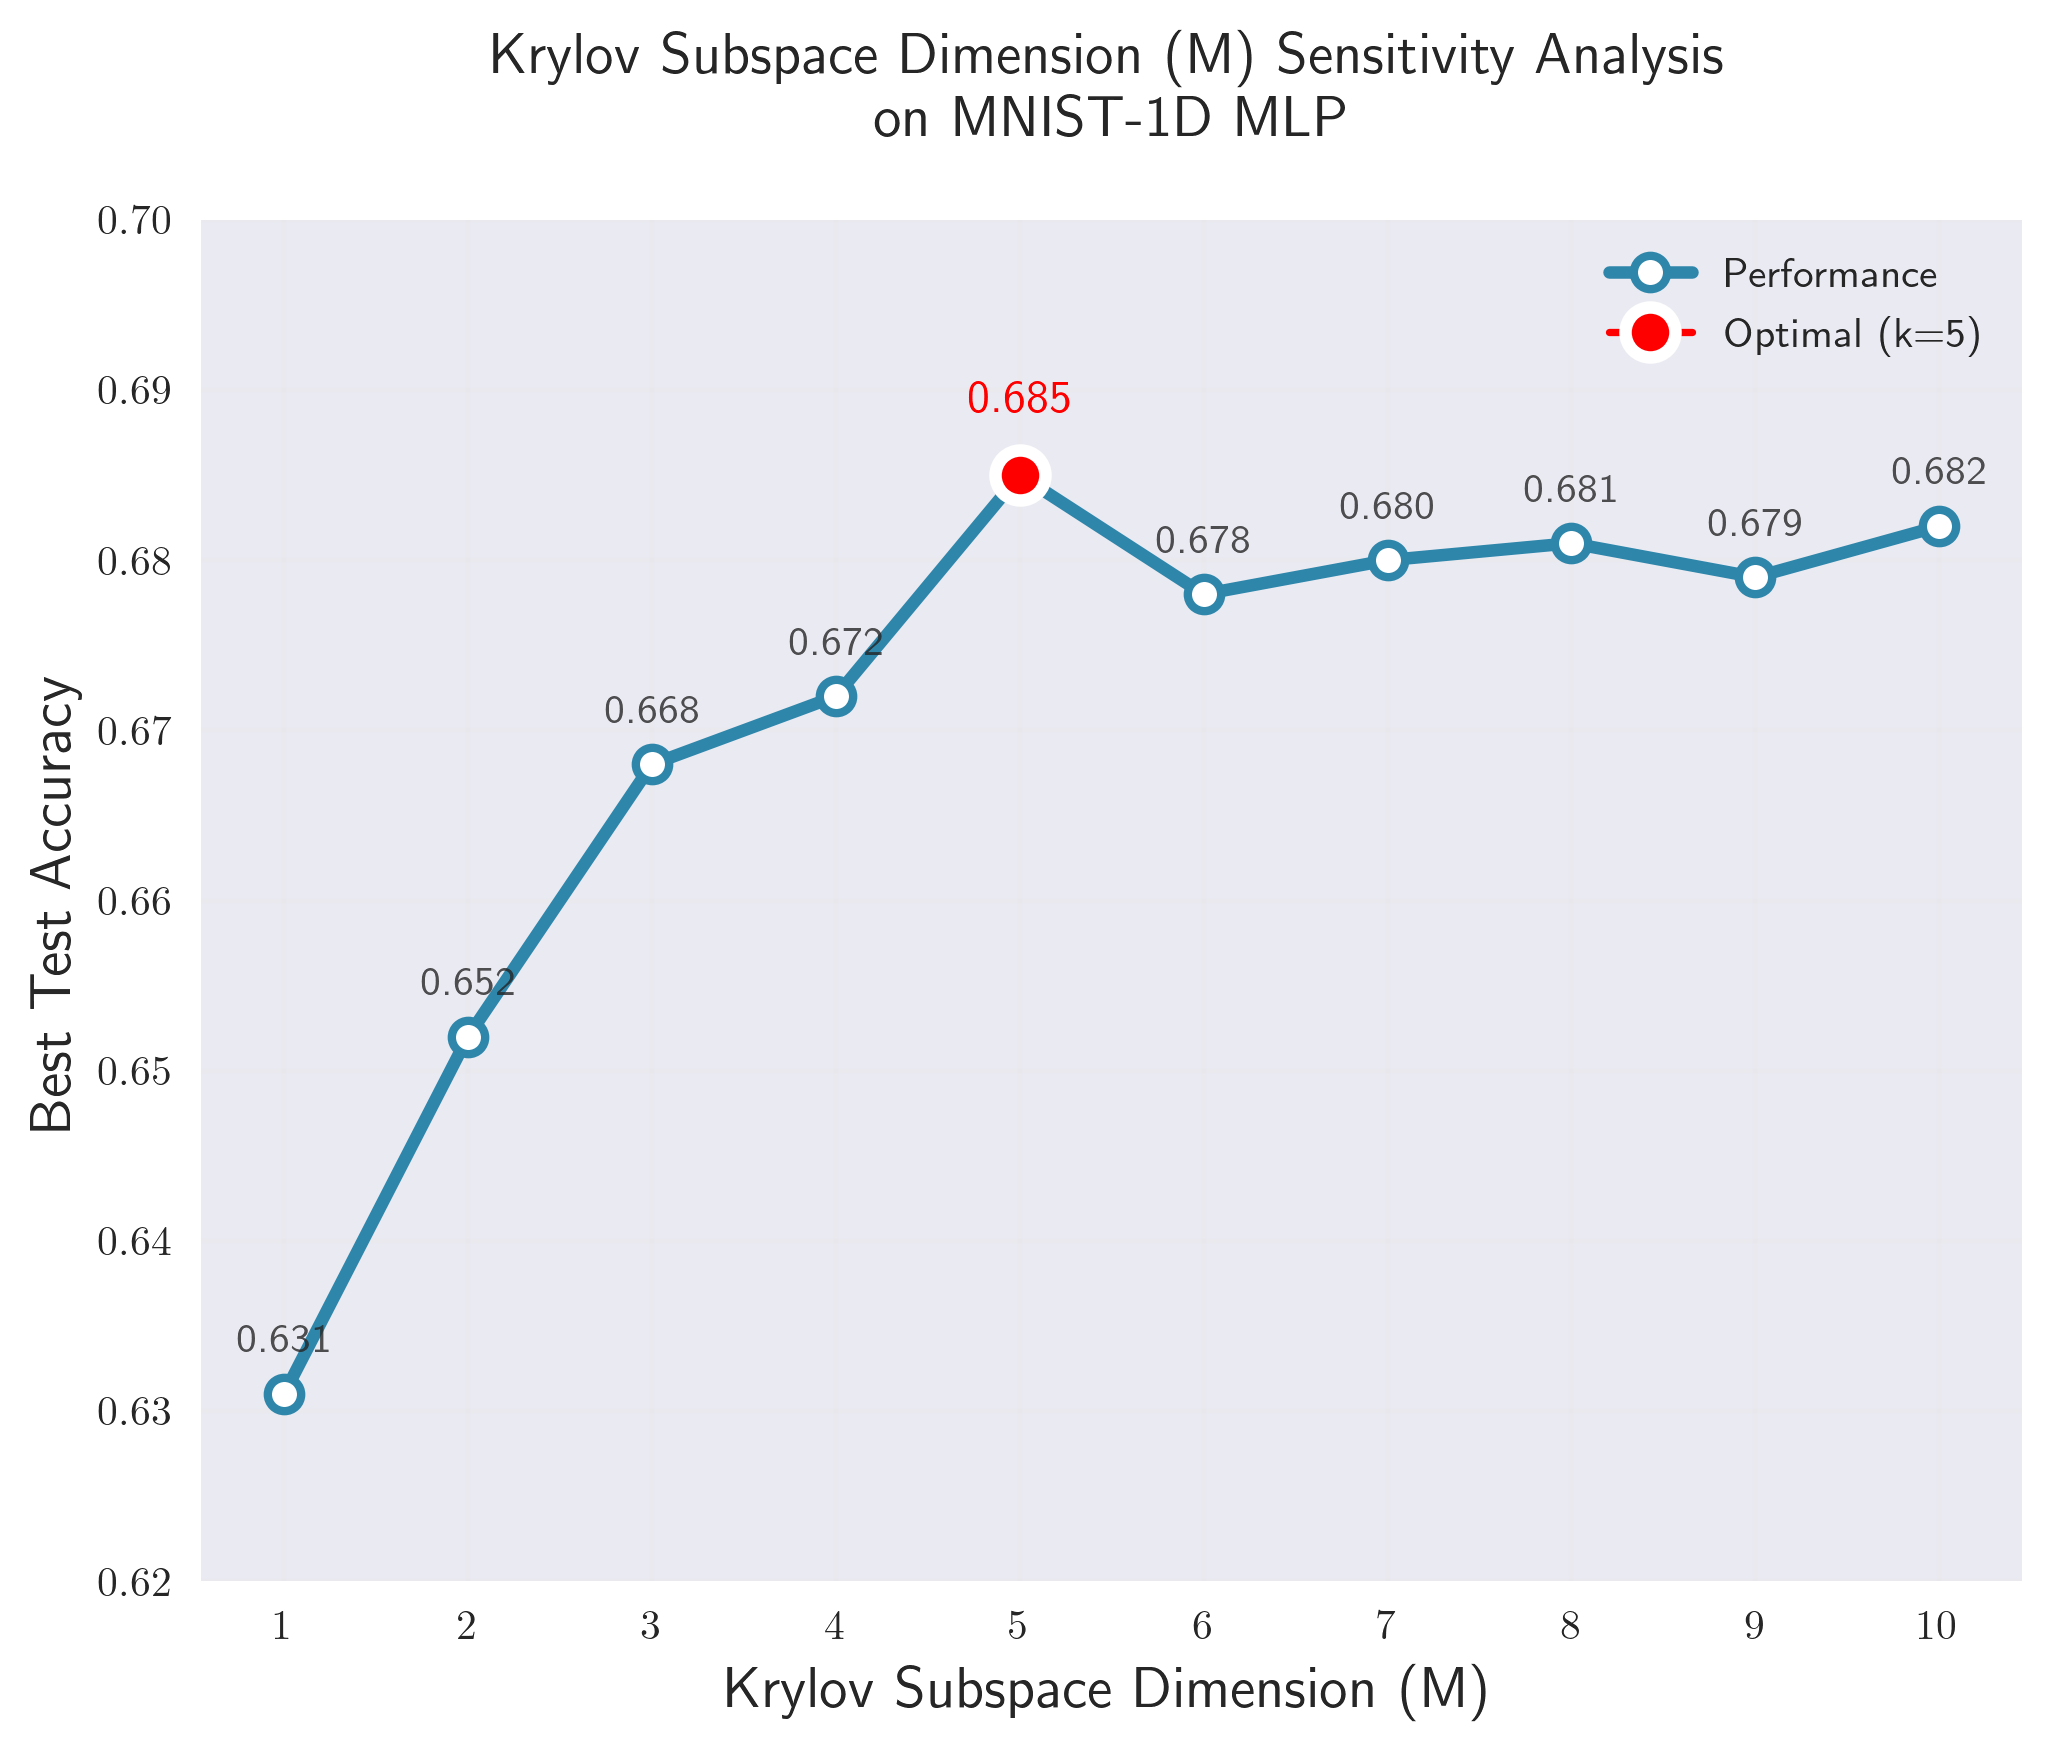
\includegraphics[width=\linewidth]{figures/5evals/sens_krylov_dim.png}
        \caption{The sensitivity analysis of the Krylov subspace dimension $M$ on MNIST-1D MLP.}
        \label{fig:sens_krylov_dim}
    \end{subfigure}
    \hfill
    \begin{subfigure}[b]{0.49\linewidth}
        \centering
        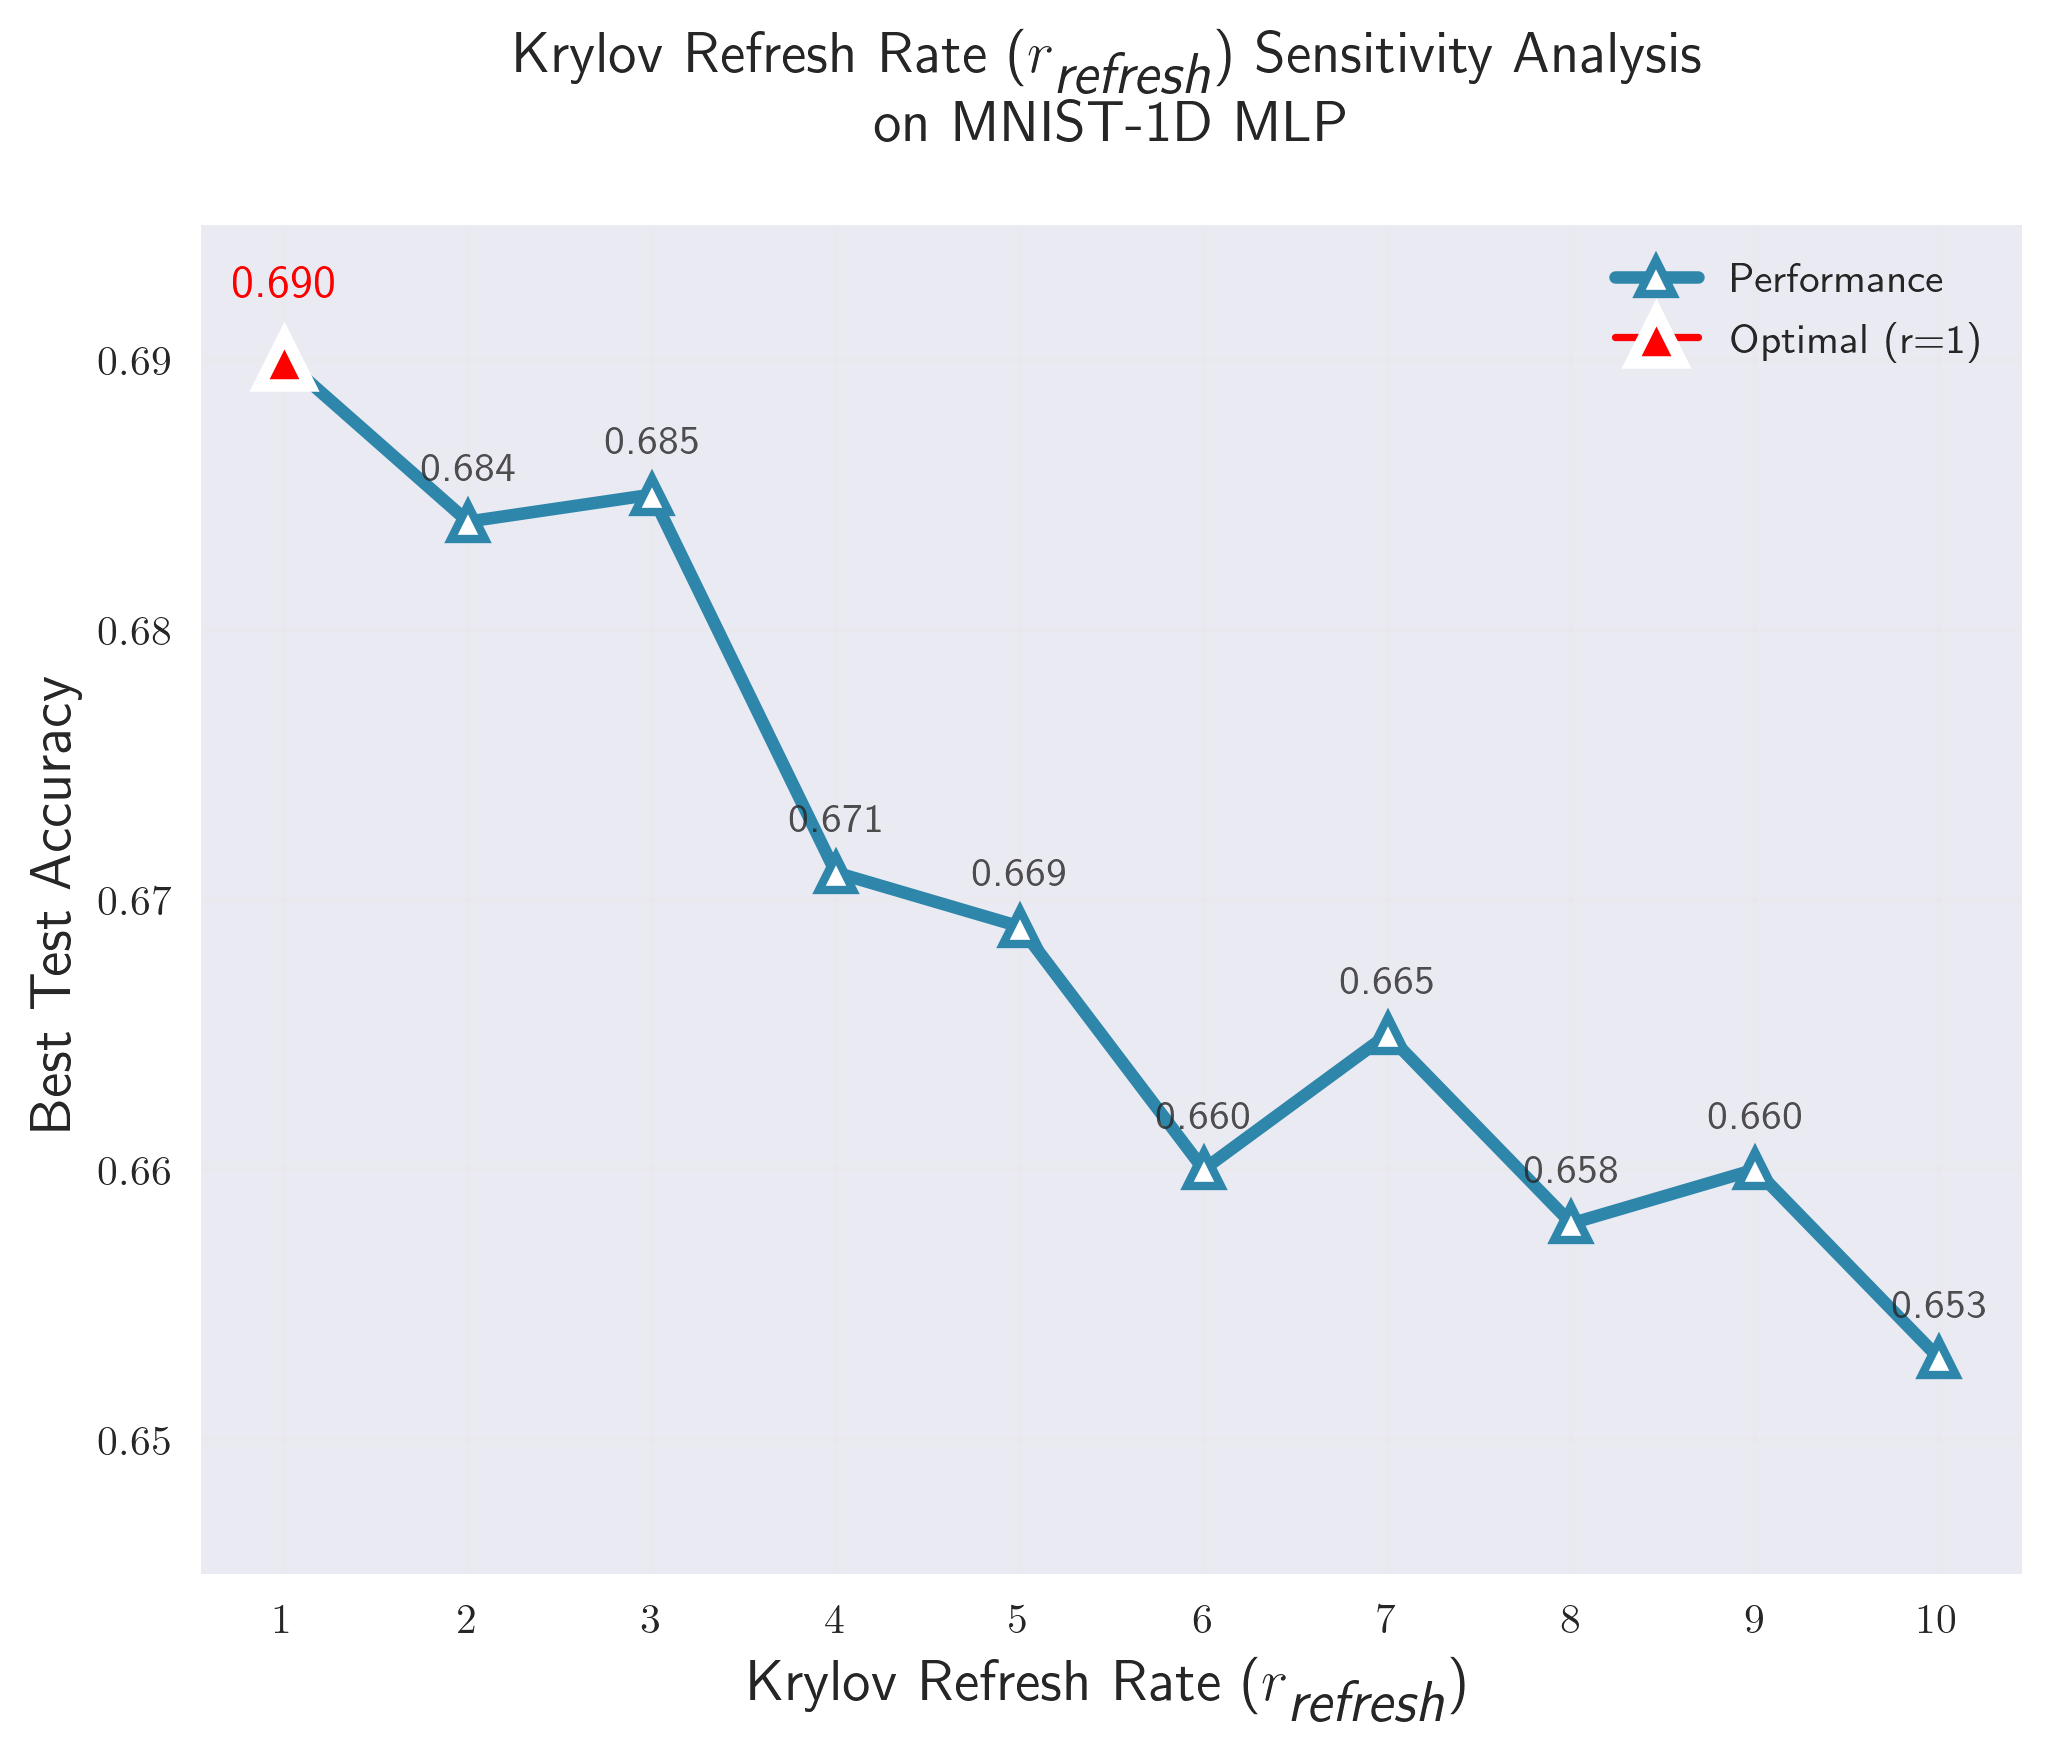
\includegraphics[width=\linewidth]{figures/5evals/sens_refresh.png}
        \caption{The sensitivity analysis of the krylov refresh rate $r_{\mathit{refresh}}$. on MNIST-1D MLP.}
        \label{fig:sens_r_refresh}
    \end{subfigure}
    \caption{Sensitivity analysis of KryBall on the MNIST-1D MLP task. We vary the Krylov dimension $M$, the maximum trust region radius $\Delta_{\mathit{max}}$, and the krylov refresh rate $r_{\mathit{refresh}}$. The parameters are varied according to their hyperparameter ranges we defined in \cref{ssec:sensitivity_analysis}. The best performing point is marked in red.}
    \label{fig:sensitivity_analysis}
\end{figure}

\textbf{Krylov Subspace Size $(M)$}: We see that the Krylov subspace size $M$ is sensitive to the performance of KryBall. For low $M$, performance suffers since we are not able to approximate the Hessian well. As $M$ increases, we obtain good performance. However, as we continue to increase $M$ past a certain point (5), our performance plateaus. This is interesting, as usually a higher $M$ results in a better approximation. We suspect that for $M=5$ onwards, the dominant curvature information has already been captured. The new basis vectors that are generated are less relevant and do not add useful information, since we have already captured most of the curvature information previously. We present some further analysis about our approximation in \cref{sec:discussion_and_further_analysis}.
 
\textbf{Krylov Refresh Rate $(r_{\mathit{refresh}})$}: The Krylov refresh rate is best when $r_{\mathit{refresh}} = 1$. This is because when $r_{\mathit{refresh}} = 1$, we use compute the Krylov subspace at every single iteration and are always using the most information. As $r_{\mathit{refresh}}$ increases, we instead fall back to our approximation not at the current point in the optimisation landscape. This is fine if we our information is not too outdated, as is the case for $r_{\mathit{refresh}} = 2$ and $r_{\mathit{refresh}} = 3$. However, as $r_{\mathit{refresh}} \geq 4$ our information is outdated and thus our quadratic model approximation is no longer accurate. This results in KryBall performing worse. We choose $r_{\mathit{refresh}} = 3$ as our default value.

\section{Discussion and Further Analysis}
\label{sec:discussion_and_further_analysis}

In this section, we present critical questions about the results we have observed and the choices we have made in evaluating our algorithm. We then answer these questions with hypotheses, experiments and further analysis. 

\textbf{Why do we see late epoch instability but good early epoch performance?}

We saw in \cref{ssec:results_image_classification} that KryBall achieves good early epoch performance, but late epoch instability. We suspect this has to do with our quadratic approximation. In the early epochs, our quadratic model is accurate and a good approximation of the landscape. However, as training progresses, the landscape changes and we suspect that a quadratic model is less accurate. 

\cite{ma2022beyond} state that the loss landscape of neural networks is multiscale, and that the quadratic model is only a local approximation of the landscape. Specifically, they find that in a neighbourhood of the local minima, the loss mixes a continuum of scales and instead grows subquadratically. As dimensionality increases, they state that the loss landscape instead shows several separate scales. This means that our quadratic model is not accurate in the presence of local minima. Given that the loss landscape is multiscale, and more importantly subquadratic near the local minima, this means that a first-order approximation may be better. In \cref{fig:cifar10_cnn_acc} and \cref{fig:cifar10_resnet_acc}, it is plausible that the variance we see near the end of training is due to this. 

To illustrate this, we perform a small experiment. We take the MNIST-1D MLP model with SGD and at distinct points in the training process, we sample the loss landscape. This is done through an exhaustive line search over $\lambda \in [-2, 2]$. We then plot what the loss landscape is at the start and end of training. This empirically shows a slice of the loss landscape from the perspective of SGD. 

\begin{figure}[!t]
    \begin{subfigure}[b]{0.49\linewidth}
        \centering
        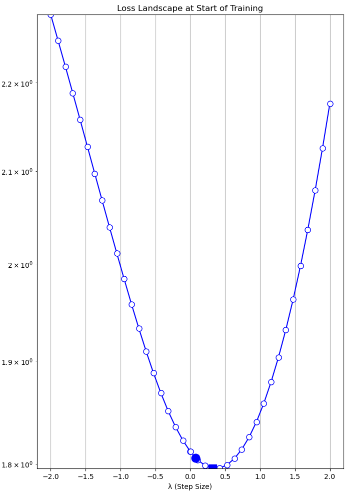
\includegraphics[width=\linewidth, height=0.4\textheight]{figures/5evals/ll_sgd_start.png}
        \caption{The loss landscape at the start of training (first epoch).}
        \label{fig:ll_sgd_start}
    \end{subfigure}
    \hfill
    \begin{subfigure}[b]{0.49\linewidth}
        \centering
        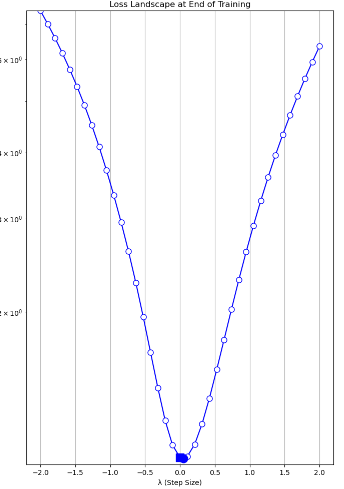
\includegraphics[width=\linewidth, height=0.4\textheight]{figures/5evals/ll_sgd_end.png}
        \caption{The loss landscape near the end of training (last epoch).}
        \label{fig:ll_sgd_end}
    \end{subfigure}
    \caption{The loss landscape of the MNIST-1D MLP model from the view of SGD.}
    \label{fig:ll_landscape}
\end{figure}

At the start of training, we see that the landscape is shaped exactly like a quadratic bowl in \cref{fig:ll_sgd_start}. However, near the end of training, that the landscape is approximately quadratic instead as seen in \cref{fig:ll_sgd_end}. It no longer is shaped exactly like a quadratic, but instead is stretched inwards. This agrees with \cite{ma2022beyond}, and it is plausible that this shape is similar to that of a subquadratic landscape.

\textbf{What is the effect of the activation function on our optimiser?}

All classification tasks in \cref{ssec:results_xor_classification} and \cref{ssec:results_image_classification} are evaluated with the Softplus activation function. Now, we examine the effect of the activation function on our optimiser. We evaluate the MNIST-1D MLP task with the following different activation functions using KryBall: ReLU, Softplus, Tanh and GeLU.

\begin{figure}[!t]
    \begin{subfigure}[b]{0.49\linewidth}
        \centering
        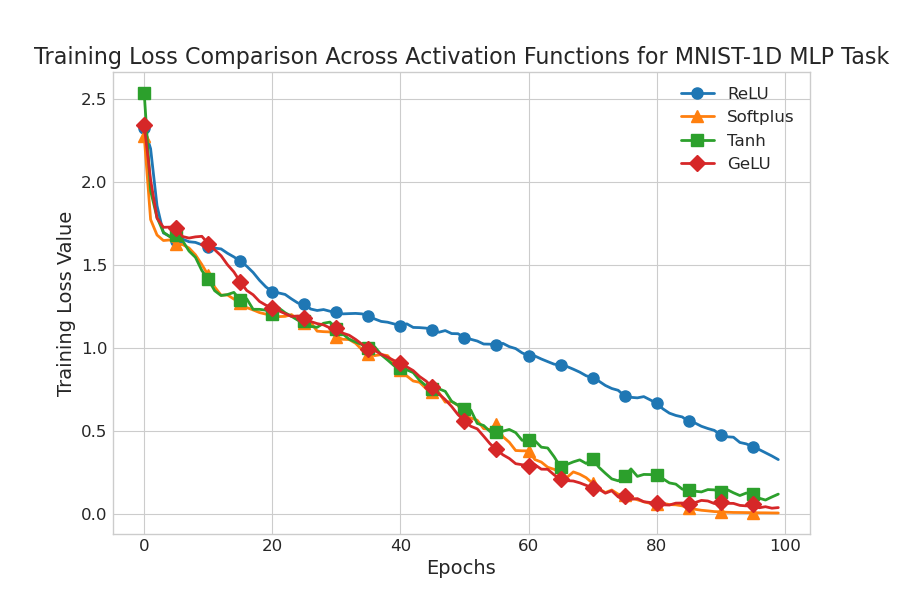
\includegraphics[width=\linewidth]{figures/5evals/mnist1d_activation_loss.png}
        \caption{Loss curves of the MNIST-1D MLP task with different activation functions using KryBall.}
        \label{fig:act_loss}
    \end{subfigure}
    \hfill
    \begin{subfigure}[b]{0.49\linewidth}
        \centering
        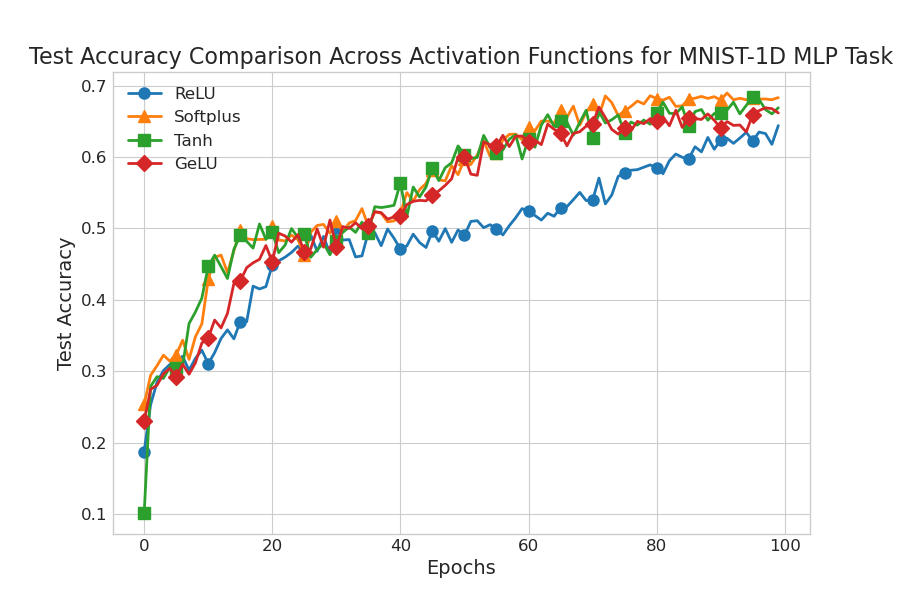
\includegraphics[width=\linewidth]{figures/5evals/mnist1d_activation_acc.png}
        \caption{Test accuracy of the MNIST-1D MLP task with different activation functions using KryBall.}
        \label{fig:act_acc}
    \end{subfigure}
    \caption{The loss curves and test accuracy of the MNIST-1D MLP task evaluated with KryBall and ReLU, Softplus, Tanh and GeLU activation functions.}
    \label{fig:act_results}
\end{figure}

In \cref{fig:act_results}, there is a stark distinction between the smooth activations and the non-smooth activation function ReLU. When using smooth activation functions, we reach close to training loss and our test accuracy is much better. However, the loss is much higher and our accuracy is lower when using ReLU. We have a good reason for this, which is that the quadratic approximation suffers in the presence of non-smooth activation functions. ReLU introduces non-differentiability at zero. This means that our quadratic model and trust-region framework, whose underlying assumptions are that we operate in smooth regions, is violated. Our method relise on meaningful HVPs for the approximation, but these are not well-defined at the transition points of ReLU units. This leads to poor curvature approximations.At this point, if we try to approximate the Hessian and the surrounding region using a quadratic model, we ultimately will not be able to. As such, it is better to use first-order methods that do not have these assumptions when using non-smooth activation functions. 

\textbf{Are our directions meaningful and distinct?}

\cite{tinysubspaces} show that gradients exhibit spurious alignment with the dominant eigenspace of the Hessian during training. Specifically, when the gradient appears to align with the top eigenspace, projecting it onto this subspace actually yields poor training progress \cite{tinysubspaces}. This finding suggests that our construction of distinct search directions is likely meaningful. Our method explicitly constructs directions from different sources. The SFN step, where we apply the $\abs{\cdot}$ function to the eigenvalues, alters the dominant subspace by ensuring positive definiteness. We hypothesis that this likely breaks the spurious alignment observed in standard training, making our dominant eigenspace directions genuinely useful rather than being correlated with the gradient. The strong empirical performance of KryBall on ill-conditioned problems, where eigenspace structure is critical. This supports the hypothesis that our multi-directional search strategy captures meaningful aspects of the optimisation landscape that individual directions cannot provide alone.

\textbf{How can we tell if our computed SFN step approximates the true SFN step?}

The crux of the Krylov subspace approach is to approximate the Hessian with a low-dimensional projected Hessian that lets us compute the SFN step. We now quantify how to analytically measure this approximation quality through the reconstruction error
\begin{align}
    ||r|| = ||z^* - \hat{z}||,
\end{align}
where $z^*$ is the true SFN direction and $\hat{z}$ is our Krylov approximation:
\begin{align}
    \hat{z} = \sum_{k=0}^{m-1} \alpha_k H^k \hat{g}.
\end{align}
Using the eigendecomposition $H = V \Lambda V^T$ and letting $c = V^T \hat{g}$, we can express both directions in terms of the eigenvalues. The true SFN direction becomes:
\begin{align}
    z^* = -V |\Lambda|^{-1} c,
\end{align}
while our Krylov approximation can be written as:
\begin{align}
    \hat{z} = V \left(\sum_{k=0}^{m-1} \alpha_k \Lambda^k\right) c.
\end{align}
We can then minimise the reconstruction error by formulating it as a linear system.
\begin{align}
    r &= z^* - \hat{z} = V(-|\Lambda|^{-1} - \sum_{k=0}^{m-1} \alpha_k \Lambda^k)c
\end{align}
We can minimise $r$ by setting the middle term to zero, in which we get,
\begin{align}
    &\Rightarrow -|\Lambda|^{-1} = \sum_{k=0}^{m-1} \alpha_k \Lambda^k \\
    &\Rightarrow -|\lambda_i|^{-1} = \sum_{k=0}^{m-1} \alpha_k \lambda_i^k \quad \text{for each eigenvalue } \lambda_i \\
    &\Rightarrow M\alpha = -1_r \quad \text{where } M_{i,k} = |\lambda_i| \lambda_i^k.
\end{align}
Solving this linear system for $\alpha$ and computing $||r||$ tells us how well our basis represents the ideal $|\Lambda|^{-1}$ operator. A small reconstruction error indicates that our limited Krylov subspace adequately spans the directions needed for an accurate SFN step. A large reconstruction error indicates that at the current point, our computed SFN step is not a good approximation of the true SFN step. Thus, we can use this to monitor the quality of our SFN step.

\section{Limitations}
\label{sec:limitations}

While KryBall demonstrates promising performance across several optimisation tasks, our evaluation reveals important limitations. We now discuss these limitations and how to address them.

\subsection{Late-Epoch Instability}
\label{ssec:late_epoch_instability}

As demonstrated in our CIFAR-10 experiments, KryBall exhibits increased variance and instability in later training epochs. This occurs when the quadratic approximation becomes less accurate near local minima, where the loss landscape exhibits multiscale, subquadratic behaviour \citep{ma2022beyond}. We also saw empirical evidence of this when we sampled the optimiser trajectory in \cref{fig:ll_landscape}. One way to address this is to switch off the quadratic model and only use first-order information as we approach the local minima. This would likely require a heuristic where after a certain point in training, we switch off the quadratic model and only use either SGD or Adam. This is a hybrid approach, and we discuss this further in \cref{ssec:hybrid_approaches}.
    
\subsection{Dependence on Smooth Activation Functions}
\label{ssec:dependence_on_smooth_activation_functions}

A fundamental limitation of KryBall is that it requires smooth activation functions to operate effectively. Our analysis in \cref{fig:act_results} shows that non-smooth activation functions such as ReLU significantly degrade performance, as points of non-differentiability violate the underlying assumptions of the quadratic model. To address this, we require a way to approximate these points without using the quadratic model. Approximation by finite differences is one such method. This has been done by \cite{finite_diff} to approximate the Hessian cheaply, and has shown to be effective in CIFAR-10 classification tasks.

\subsection{Hyperparameter Sensitivity}
\label{ssec:hyperparameter_sensitivity}

Our sensitivity analysis reveals that KryBall is reasonably sensitive and dependent on the Krylov dimension $M$ and refresh rate $r_{\text{refresh}}$. We note that while our hyperparameters are not as sensitive as Adam and MSGD, they still require careful tuning, where suboptimal values can lead to poor performance as we saw in \cref{fig:sensitivity_analysis}. One way to address this could be to use adaptive schemes that automatically adjust $M$ and $r_{\text{refresh}}$. This has been done by \cite{henriques2019small}, who automatically rescale hyperparameters by using an objective change heuristic.

\subsection{Trust-Region Step Rejection}
\label{ssec:trust_region_step_rejection}

Our trust-region framework can reject optimisation steps when the quadratic model poorly predicts actual function behavior. While this provides stability, frequent step rejections can slow convergence compared to first-order methods that always accept their steps. This is particularly the case when the Hessian approximation degrades or is in highly non-quadratic regions. A good way to address this is to simply use the gradient or momentum as a fallback. Moreover, we can instead consider a hybrid approach where if our step is rejected, we proceed with a first-order optimiser such as Adam or MSGD.

\subsection{Computational Overhead}
\label{ssec:computational_overhead}

KryBall requires computing HVPs and constructing Krylov subspaces, introducing additional computational cost compared to first-order methods. While HVPs can be computed efficiently using automatic differentiation, the overall cost per iteration remains higher than gradient-only approaches. The key limitation here is that the main computational cost comes from the construction of the Krylov subspace, as our Krylov dimension $M$ is fixed throughout training. This overhead could be mitigated by adaptively reducing the Krylov dimension $M$ in regions where high-quality approximations are not critical, or by increasing the refresh rate $r_{\text{refresh}}$ when the landscape is relatively stable.

In this section, we presented the evaluations of our optimiser, KryBall, on a range of tasks. We evaluated KryBall's performance on ill-conditioned problems, simple binary classification, and more complex image classification tasks. We discussed KryBall's performance in comparison to the state-of-the-art optimisers Adam and MSGD. We then followed with a sensitivity analysis, a deeper discussion about key questions and finally the limitations of our method. We now move on to conclude this thesis.